%%% mythesis.tex
%%
%% this file, mythesis.tex, is the main file of a fictitious
%% Penn State Ph D thesis 
%%
%%% 
%% this material can be used as a template to prepare your own Ph D thesis
%%
%% this file was created Sept 1995 by Stephen G. Simpson,
%% simpson@math.psu.edu
%%
%% revised November 1996, S. Simpson
%% revised 2002, Sarah Gallager (to allow deluxetables)
%% modified a little more by Michele Stark (2004)

\documentclass[10pt,rmp,aps]{psuthesis}

%% optional packages, in case you want AMS math macros and AMS symbols
\usepackage{amsmath,amssymb}
%% allows bibtex, \citet{}, \citep{} referencing:
%\usepackage{natbib}
%% I truthfully don't know what the following is for, but I never used it:
%\citestyle{aa}
%% optional package, in case you want PostScript graphics:
\usepackage{graphicx} 

\DeclareGraphicsExtensions{ .png, .pdf, .jpg }

\usepackage{subfigure}
%
%% the following allows you to use the AAS deluxetable environment:
%\usepackage{deluxetable}
%% Use the following if you have tables that are longer than a single page::
%\usepackage{longtable}
%% Use the following if you have (non-deluxetables, i.e., longtables) that
%% you need to display landscape oriented:
%\usepackage{lscape}

\usepackage{wick}
%\usepackage[dvipdfm]{graphicx}
%\usepackage{epsfig}
\usepackage[pdftex]{hyperref}

\hypersetup{
%    bookmarks=true,         % show bookmarks bar?
%    unicode=false,          % non-Latin characters in Acrobats bookmarks
%    pdftoolbar=true,        % show Acrobats toolbar?
%    pdfmenubar=true,        % show Acrobats menu?
%    pdffitwindow=false,     % window fit to page when opened
%    pdfstartview={FitH},    % fits the width of the page to the window
%    pdftitle={My title},    % title
%    pdfauthor={Author},     % author
%    pdfsubject={Subject},   % subject of the document
%    pdfcreator={Creator},   % creator of the document
%    pdfproducer={Producer}, % producer of the document
%    pdfkeywords={keywords}, % list of keywords
	%    pdfnewwindow=true,      % links in new window
%    colorlinks=true,       % false: boxed links; true: colored links
    linkcolor=black,          % color of internal links
    citecolor=green,        % color of links to bibliography
    filecolor=magenta,      % color of file links
    urlcolor=cyan           % color of external links
}

%Deepak's custom commands
\usepackage{parskip}
%\setlength{\parindent}{0in}
%\usepackage{setspace}

%% for a less-than-final version of the thesis
%\thesisdraft    
%% comment this out for the final version

%% you can speed things up by compiling only one chapter at a time
%\includeonly{chapters/intro}
%\includeonly{chapters/voids_vs_lcdm}
%\includeonly{someotherchapter}
%\includeonly{yetanotherchapter}
%\includeonly{Ithinkyougettheideachapter}
%\includeonly{conclusions}
%% comment this out for the final version

%% Fix the text citations so that there is no comma between the authors and 
%% year.  This will help contain the furious Brandt red pen.
%\bibpunct{(}{)}{;}{a}{}{,}

%% Change the fonts back to something reasonable.
%% Note: scriptsize is typically smaller than footnotesize.
%\renewcommand{\scriptsize{\@setfontsize\scriptsize\@ixpt{9pt}}
%\renewcommand{\footnotesize{\@setfontsize\scriptsize\@xpt{10pt}}

%%
%% These are all the definitions that I've used throughout my thesis.
%\input{../articles/my_definitions.tex}

%%% Custom commands %%%
\newcommand{\bite}{\begin{itemize}}
\newcommand{\eat}{\end{itemize}}
\newcommand{\beq}{\begin{equation}}
\newcommand{\eeq}{\end{equation}}
\newcommand{\rarrow}{\rightarrow}
\newcommand{\bra}{\langle}
\newcommand{\ket}{\rangle}
\newcommand{\beqa}{\begin{eqnarray}}
\newcommand{\eeqa}{\end{eqnarray}}
\newcommand{\barr}{\begin{array}}
\newcommand{\earr}{\end{array}}
\newcommand{\del}{\partial}
\newcommand{\de}{\mathrm{d}}
%\newcommand{\mu\nu}{{\mu\nu}}
\renewcommand{\th}{\mathrm{th}}
\newcommand{\com}[1]{\begin{itemize}\color{RED}{{#1}}\end{itemize}}
\newcommand{\C}{\mathbb{C}}
\newcommand{\R}{\mathbb{R}}
\newcommand{\btw}[1]{\color{PURPLE}{{#1}}\color{BLACK}}
\newcommand{\cut}[1]{\color{RED}{{#1}}\color{BLACK}}

\newcommand{\mb}[1]{\mathbf{#1}}
\newcommand{\mc}[1]{\mathcal{#1}}
\newcommand{\mbb}[1]{\mathbb{#1}}
\newcommand{\mf}[1]{\mathfrak{#1}}

\newcommand{\vectb}[1]{\matbf{\vec{#1}}}
\newcommand{\vecta}[1]{\overrightarrow{#1} }
\newcommand{\vect}[1]{\boldsymbol{#1}}
\newcommand{\expect}[1]{\langle #1\rangle}
\newcommand{\innerp}[2]{\langle #1 \vert #2 \rangle}
\newcommand{\fullbra}[1]{\langle #1 \vert}
\newcommand{\fullket}[1]{\vert #1 \rangle}
\newcommand{\supersc}[1]{$^{\textrm{#1}}$}
\newcommand{\subsc}[1]{$_{\textrm{#1}}$}
\newcommand{\sltwoc}{\mathfrak{sl}(2,\mathbb{C})}

\begin{document}

%%Comment this out for the final thesis:

%%

%% at the beginning of the thesis we have a title page, a signature
%% page, and an abstract

\author{Deepak Vaid}


\title{\uppercase {The Cosmological Constant\\and \\
       Many-Body Physics: An Investigation}}

\dept{Physics}

\submitdate{October 2010}

\copyrightyear{2010}


\begin{singlespace}

\readerone{Stephon Alexander\ Member1\\
	 \adviser \\
	 \cochair \\
           Assistant Professor (adjunct) of Physics \\
           \assocprof{Physics, Haverford College}}

\readertwo{Martin Bojowald\\
         \assocprof{Physics} \\
         \chair}

\readerthree{Jainendra Jain\ Member2 \\
             Erwin W. Mueller Professor of Physics}

\readerfour{Peter Meszaros\ Member3 \\
             Eberly Chair of  Astronomy \& Astrophysics\\
             Professor of Physics}

\readerseven{Jayant Bhanavar\\
             \prof{Physics}\\
             George A. and Margaret M. Downsbrough Department Head of Physics}

%%%   Key to titles:
%%% Associate Professor: \asocprof{of what}
%%% Assistant Professor: \assistprof{of what}
%%% Full Professor: \prof{of what}
%%% also Dept. Head: \head{of what}
%%% You can also do things like: ``Associate \head{of what}''

\begin{frontmatter}

%\begin{doublespace}
\titlepage
%\end{doublespace}

% committee page (signature page has been discontinued)
\vbox{
    \thispagestyle{empty}
    \begin{singlespace}
    \hbox{The dissertation of Deepak Vaid was reviewed and approved${}^\ast$ by the following:}
    \vskip 0.5in
    Stephon Alexander\\\
           Assistant Professor (adjunct) of Physics \\
           \assocprof{Physics, Haverford College\\
           \adviser \\
	 \cochair}
     \vskip 0.5in
     Martin Bojowald\\
         \assocprof{Physics} \\
         \chair
     \vskip 0.5in
     Jainendra Jain\  \\
             Erwin W. Mueller Professor of Physics
     \vskip 0.5in
     Peter Meszaros\ \\
             Eberly Chair of  Astronomy \& Astrophysics\\
             Professor of Physics
      \vskip 0.5in
      Jayant Bhanavar\\
             \prof{Physics}\\
             George A. and Margaret M. Downsbrough Department Head of Physics
    \vskip 2in
    \hbox{${}^\ast$Signatures are on file at the Graduate School} 
    \end{singlespace}
    \typeout{Signature page.}
} \newpage

%\signaturepage

%\end{singlespace}

\abstract

A model for condensation of fermions in a flat Friedmann-Robertson-Walker (FRW) background is presented. It is shown that condensation can happen, via the BCS mechanism due to a four-fermion interaction which appears naturally when fermions are included in gravity. We argue that this process can form the basis for a non-perturbative resolution to the cosmological constant problem. In order to make contact with observational evidence, we show that CMB data from the WMAP3 mission can be fitted to a cosmological model with zero $\Lambda_{eff}$, provided that we live in a universe riddled with voids of the order of ~100 Mpc. For our calculations voids are approximated by LTB metrics. We argue that the correct way to model voids is based on the methods of dark matter structure formation, which are highly non-linear but are amenable to an analytic treatment.

%% this is the end of the abstract

%% after the abstract come the table of contents, the list of tables,
%% and the list of figures
%% Note about the figure list... so the figure list is a decent length,
%% use the following command for the figure captions:
%% \caption[Short figure title to appear in figure list]{Normal figure caption}
%% (this trick unfortunately does not work with the deluxetable 
%% ``\tablecaption'' command, so be careful what you put in the table captions)
%%
%% If you have really long tables that cover multiple pages, you
%% will want to use the ``longtable'' environment (it is very similer to
%% deluxetable) but allows you to specify headers and footers for the first,
%% last, and middle pages of the figure.

%% use this command to omit the list of tables,
%% if the thesis doesn't contain any tables
%\nolotables

%% use this command to omit the list of figures,
%% if the thesis doesn't contain any figures
%\nolofigures

\tables

%% next come the acknowlegements (optional) and the preface (optional)

\acknowledgments  % optional

This work was made possible by all the people who had faith in me when I doubted myself, who lifted me when I was down and who inspired me when I felt lost. They include:

George Peter - a teacher extraordinaire, a kind and inspiring man who not only provided moral ballast at a crucial time in my life but also encouraged me to stick to my chosen path;

my high school math teacher - another great educator who recognized the stifling effect schools can have on a young individuals creativity and ambition and therefore nurtured the same in me;

Narendra Srivastava - an artist, a genius and a man of great wisdom with whom I shared many evenings playing chess and talking about physics, philosophy and life;

Shubranghsu Sengupta (Rushi) - my friend and confidante who first introduced me to the wonderful world of physics;

Sat Pal Kalra - for feeding a youngster's zeal for knowledge and inspiration with subscriptions to Scientific American and books such as \emph{A Brief History of Time};

Stephon Alexander - a brilliant physicist, my advisor and guiding light as a graduate student;

Martin Bojowald - another physicist \emph{par excellence} whose decision to serve as my committee chair was a life-saver;

the State College "gang" consisting of Vinay Kumar, Lisa Santini, Megan Broda, Whitney Polakowski, Renae DiPierre, Nathaniel Hermann, Eric Goeller, Rusty Andrews, Sean Brinza, Sarah Catalina, Darcy Worden, Aarao Cornelio and many others who were my friends in turbulent times;

the secretaries and administrative assistants who greased the wheels of beauracracy and assisted me on numerous occasions with missed deadlines and missing forms;

and finally my parents and my family, immediate and extended, the people who at each step in my life stood by me even as I tested their patience and reserves of love sorely and to whom this thesis is dedicated.

%\preface    % optional

\clearpage

\vspace*{2.0truein}

%\LARGE
\parbox{4.0truein}{
\par\noindent
Let no man ignorant of Geometry enter here\\
\hspace*{\fill}--Plato.
}
\normalsize

\vspace*{2.0truein}

%\LARGE
\parbox{4.0truein}{
\par\noindent
And I cherish more than anything else \\
\hspace*{0.5 in}the Analogies, my most trustworthy masters. \\
They know all the secrets of Nature, \\
\hspace*{0.5 in}and they ought least to be neglected in Geometry.\\
\hspace*{\fill}--Johannes Kepler
}

%All this has happened before, and all this will happen again\\
%\hspace*{\fill}--Battlestar Galactica.

\end{frontmatter}

%% this is the end of the front matter

%% now we include the actual chapters of the thesis
%% there are individual chapter files ch-intr.tex, ch-over.tex, ...
%% (NOTE: you do not need the ``.tex'' extention on the file name
%% in the include statement)
%% these chapters can be in a sub-directory, for example: 
%% \include{chapterdirectory/chaptername}

\chapter{Cosmological Considerations}

\begin{doublespace}

\section{A Brief History of Cosmology}

Cosmology is one of the oldest and perhaps the grandest of human sciences.
The word \char`\"{}cosmos\char`\"{} is commonly understood to represent
the entire Universe. It originates from the Greek word for order i.e.
the opposite of chaos and disorder \cite{Wikipedia2008Cosmology}. Since
ancient times, across history and all civilizations the human mind
has always been drawn to the night sky and to the order apparent in
it. What, our curiosity compels us to ask, is the mechanism that causes
this Order to come about, not only in our planetary sphere but on
the scale of the stars and galaxies? Today the word {}``cosmology''
has a somewhat narrower interpretation in terms of the study of the
dynamics of the Universe in the language of physics and mathematics,
but though the language might have become more structured the essential
question remains the same.

The first viable mathematical description of a cosmological model
was possible only after the discovery of General Relativity by Albert
Einstein\cite{Einstein:1920RelativityBook}, a framework which allows
us to describe the motion not only of matter but also of the spacetime
manifold in which matter lives. Even though Einstein himself, for
personal and aesthetic reasons, was a proponent of a static universe,
the discovery of solutions for expanding cosmological metrics by DeSitter,
Freidmann, Le'Maitre and others pointed elsewhere. The discovery of
the redshifting of the spectra of distant nebulae and galaxies by
Edwin Hubble in 1920\cite{Hubble:1929PNAS} provided concrete evidence
for an expanding universe. This discovery raised even more vexing
questions. If the Universe is expanding in the present epoch then
at some earlier epoch all the matter and energy must have existed
in the form of an incredibly dense and hot Cosmic egg. This birthing
scenario for the Universe came to be known as the {}``Big Bang''
hypothesis. At this stage not only gravitational but also quantum
mechanical fluctuations would become significant. Thus a theory of
{}``quantum gravity'' would necessarily be required to properly
describe the earliest epoch of the Universe. Consequently research
in theoretical cosmology since the 1930s until the present has essentially
been a quest for such a unification of the two pillars of modern physics:
Quantum Mechanics and General Relativity.

The lack of a complete understanding of such a unification becomes
stark when considering one of the key elements of General Relativity
as formulated by Einstein - the Cosmological Constant (CC). Einstein
originally introduced this parameter into his field equations in order
to obtain a static cosmological solution which as mentioned above
seemed most natural to him. Including this term the field equations
become \cite{Wald1984General}:

\begin{equation}
G_{\mu\nu}=8\pi G\; T_{\mu\nu}-\Lambda\: g_{\mu\nu}\label{eq:GRFieldEqn}
\end{equation}


where $G_{\mu\nu}$ is the Einstein tensor, $T_{\mu\nu}$ is the matter
stress-energy tensor, $g_{\mu\nu}$ is the metric tensor and $\Lambda$
is the CC. Now the simplest form for $T_{\mu\nu}$ is that of a perfect
fluid:

\begin{equation}
T_{\mu\nu}=\rho u_{\mu}u_{\nu}+p(g_{\mu\nu}+u_{\mu}u_{\nu})\label{eq:PerfectFluidTensor}\end{equation}


where $\rho$, $P$ are the density and pressure, respectively, of
the fluid w.r.t an (unaccelerated) observer whose trajectory is given
by the four-vector $u_{\mu}$. With the CC term the effective stress-energy
tensor becomes:

\begin{equation}
T_{\mu\nu}=(\rho+p)u_{\mu}u_{\nu}+(p-\frac{\Lambda}{8\pi G})g_{\mu\nu}\end{equation}


or more explicitly for a stationary observer whose trajectory is given
by $u_{\mu}=(-1,0,0,0)$ in a flat background with metric $g_{\mu\nu}=diag(-1,1,1,1)$:

\begin{equation}
T_{\mu\nu}=\left(\begin{array}{cccc}
\rho+\frac{\Lambda}{8\pi G}\\
 & p-\frac{\Lambda}{8\pi G}\\
 &  & p-\frac{\Lambda}{8\pi G}\\
 &  &  & p-\frac{\Lambda}{8\pi G}\end{array}\right)\end{equation}


from which we can see that the CC term behaves as a perfect fluid
with energy density $\frac{\Lambda}{8\pi G}$ and \emph{negative}
pressure $-\frac{\Lambda}{8\pi G}$. This behavior is also characterized
by the \emph{equation of state}:

\begin{equation}
w=\frac{p}{\rho}\end{equation}


In the absence of any other forms of matter we have $\rho=\frac{\Lambda}{8\pi G}$
and $p=-\frac{\Lambda}{8\pi G}$, giving $w=-1$. Thus any form of
matter which has equation of state $w=-1$ has the same physical effect
on cosmological dynamics as the CC term.

For a metric parametrized by a scale factor $a(t)$ and the parameter
$k$, which takes on values $-1,0,1$ corresponding to an open (hyperbolic),
flat and closed ($S^{3}$) spatial topologies respectively:

\begin{equation}
ds^{2}=-dt^{2}+a^{2}(t)\left[ \frac{dr^{2}}{1-kr^{2}}+r^{2}(d\theta^{2}+sin^{2}(\theta)d\phi^{2}) \right]\end{equation}


and the stress-energy tensor of a perfect fluid with a CC term, only
the diagonal components of the Einstein tensor are non-zero and the
field equations reduce to \cite{Wald1984General}:

\begin{eqnarray}\label{eqn:Friedmann}
\frac{\dot{a^{2}}}{a^{2}} & = &\frac{8\pi G\rho}{3}+\frac{\Lambda}{3}-\frac{k}{a^{2}} \\
\frac{\ddot{a}}{a} & = & -\frac{4\pi G}{3}(\rho+3p-\frac{\Lambda}{4\pi G})
\end{eqnarray}


which are referred to as the first and second Friedmann equations
respectively. We can see from the first equation that for $k=+1$,
there exists a $\Lambda>0$ such that the $H^{2}=\frac{\dot{a^{2}}}{a^{2}}=0$.
For a suitable value of $p$, we can also set the RHS of the 2nd equation
to zero. This solution is known as the Einstein-static universe. It
is clear that without the presence of the CC term in the 2nd term
such a static solution would not be possible. It is an easy exercise
to show that this solution is unstable w.r.t small perturbations in
the scale factor. Therefore the Einstein-static universe, apart from
being in conflict with observation is also not a mathematically stable
solution. Thus Einstein's introduction of the CC term was a failure
in that it cannot be used to obtain a stable static solution. Subsequently
Einstein would refer to the CC term as his {}``greatest blunder''%
\footnote{Even in this {}``blunder'', Einstein had discovered a term that
lies at the crux of the clash between GR and QM and continues until
today to vex theorists and experimentalists alike with its resistance
to a final satisfactory resolution as to its physical origins and
significance.%
}.

As the focus of cosmological research moved on to the study of special
solutions of (\ref{eq:GRFieldEqn}) describing stars and black holes,
the realization of the true significance of this cosmological term
was postponed until the last decade of the 20 century when enough
evidence had accumulated from cosmological observations involving
ground and space-based platforms examples and references HST, COBE etc. to rule out all cosmological models except those with non-zero $\Lambda$ \cite{Spergel2006Wilkinson}

\subsection{Problems with FRW Models}

Though Hubble's discovery provided confirmation that the large scale structure of the cosmos was amenable to a description within the framework of Einstein's General Relativity, this was merely the beginning of the story. It was clear that the observable universe contained a great deal of structure and that any cosmological model would be considered incomplete if it did not provide some explanation as to how these large-scale inhomogeneities could form. A further layer of confusion was added by Penzias and Wilson's discovery \cite{Penzias1965A-Measurement} of the cosmic microwave background (CMB) radiation which appeared to be isotropic and uniform at a temperature of $\sim 3^{\circ}$ K, with negligible fluctuations. This radiation was the imprint of the recombination era, the time when the universe had cooled enough for electrons and protons to form hydrogen atoms. Naturally any gravitational inhomogeneities present at that epoch would have left a signature on the radiation emitted during recombination. And these same inhomogeneities constituted the seeds of present day large scale structure. However a simple calculation assuming a FRW cosmological model, shows that the structures which lie within our Hubble horizon ($\sim 3000 \, Mpc \sim 10^{26} m$) could not have been in causal contact at $t_{rec}$. How could one reconcile this observation with the observed isotropy and homogeneity of the CMB? We also happen to live in a universe with a predominance of matter over anti-matter.\footnote{The alternative would clearly be unsuitable not only for life but for any kind of stable structures such as planets and galaxies.} Now the Standard Model description of elementary particles does not incorporate CP violation, which would be required for one form of matter to be predominant. What mechanism could explain this matter-antimatter asymmetry?

\subsection{Inflationary Cosmology}

In 1982 Alan Guth, and Vilenkin and Starobinsky in the following year, proposed a new paradigm for the early universe: the inflationary model. The elegance of this solution lay in the fact that it had the potential to explain all three of the above problems (horizon/flatness problem, structure formation and matter-antimatter asymmetry) in one stroke. The idea behind inflation is simple enough. As the word implies, the universe underwent a period of exponential growth when the scale factor $a(t)$ grew as $\sim e^{-H_{inf} t}$ ($H_{inf}$ is the Hubble rate during this era) starting from some small homogenous, isotropic patch of geometry. This rapid expansion would damp out any large scale geometrical inhomogeneities present prior to inflation, avoiding the need to fine-tune the matter density at early epochs, and would naturally yield the flat, isotropic background as characterized by the CMB, leaving only small density fluctuations whose amplitude ($\delta \rho/\rho \sim 10^{-5}$) depends only on the duration of the inflationary phase. Being a non-equilibrium process, inflation provides the conditions necessary for CP violating processes to occur, which would then naturally yield an excess of particles over anti-particles.

Despite these attractive features, the biggest obstacle to accepting the validity of this model was the lack of a sensible physical mechanism. Guth's original proposal was that of \emph{false vacuum decay}. The initial state of geometry is described by a quantum state that is trapped in the false minimum of a potential. As the temperature falls, the potential is lowered sufficiently to allow the state to tunnel out resulting in bubbles of inflationary patches to grow. This model however ran into trouble because the speed of expansion of these bubbles was insufficient to allow them to combine and reach equlibrium, resulting in a highly inhomogenous universe at the end of the inflationary phase, in conflict with the homogeneity of the CMB. The other most commonly adopted class of models was based on the notion of "slow-roll". A scalar field can be shown to have a negative equation of state, the same as a positive cosmological constant and can thus drive inflation. In order to obtain the required duration of inflation, followed by a period of reheating, the potential for this scalar would in general have to have a very specific form determined by the so-called "slow-roll" conditions. The ad-hoc nature of this potential and the lack of a suitable scalar field in the Standard Model are the main deficiencies of this class of models\footnote{The SM is posited to contain the U(1) Higgs axion which is supposed to endow particles with mass via a sponatenous symmetry breaking mechanism. It is unclear however if the Higgs would correspond to the inflaton and if so how could they be related.}. In recent years, alternatives to inflation such as the ekpyrotic and bouncing universe scenarios have been proposed. String Theory has also provided fertile ground for alternatives to inflation such as the brane collision model \cite{Khoury2001Physical}. However, none of these alternatives has the simplicity and elegance of the inflationary scenario. The question then arises: can we come up with some mechanism which generates inflation without resorting to ad-hoc potentials or exotic scalar/quintessence fields which \emph{a priori} don't have sufficient grounding in our (reasonably complete) picture of the Standard Model of particles?

In this thesis, we argue that a cosmological condensate which forms via the BCS mechanism can source inflation without resort to ad-hoc potentials and also provide a resolution to the cosmological constant problem. Venturing into the speculative realm, we also conjecture that such an axion would play the role of the Higgs scalar. Inflation has the character of a phase transition. Phase transitions in particle physics are generally understood within the framework of \emph{spontaneous symmetry breaking} (SSB). An axion with U(1) symmetry could undergo SSB and be responsible for both driving inflation and endowing leptons with mass, thus playing the role of the inflaton + Higgs.

\section{Many-Body Phenomena and Gravity}

Physics has come a long way from the days of the Newtonian point particle and exactly solvable two-body systems. It is now clear that it is \emph{many body} phenomena than constitute the phenomena in Nature of deepest interest to us. Some examples of such theories are

\begin{itemize}
\item fluid-flow or hydrodynamics, under whose coarse-grained banner falls everything from the sloshing of tea in a cup to oceanic and atmospheric currents.
\item condensed matter, hard and soft, encompasses the behaviour of systems with electronic energy band structures; fermi and non-fermi liquids; excitons, polarons and other excitations in crystalline media.
\item quantum field theory, which seeks to describe the behaviour and interactions of elementary particles and gauge fields which ultimately determine the nature of the strong and electroweak forces the glue holding nuclear structure together.
\end{itemize}

In light of the arena of gravitational physics, ranging from planetary systems to galaxies, one might be tempted to think of general relativity as also being a many body phenomena. Indeed the equations of GR describe the interaction of \emph{fields} of matter and geometry, which like all fields are continuum descriptions of an underlying many body theory. However, even though the many body nature of gravitation is implicit in the structures used to define it, most physicists would initially balk at such a description.

\subsection{The Cosmological Constant term in Field Theory}

While the most concrete evidence for a non-zero $\Lambda$ has come from astronomical observations, one can also investigate this question from the perspective of local QFT and/or candidates for theories of Quantum Gravity (QG) such as LQG and String Theory. But first, let us consider the simple case of the quantum harmonic oscillator.

One of the most striking results of early quantum mechanics was Dirac's quantization of the harmonic oscillator hamiltonian is the energy eigenstate basis. The resulting hamiltonian becomes:

\begin{equation}
\hat{H} =  \hbar \omega \sum_{\vec{k}} \left( a^\dagger_{\vec{k}} a_{\vec{k}}  + \frac{1}{2} \right)
\end{equation}

where $\omega$ is the characteristic frequency of the given oscillator. This expression might seem passe to most physicists, having encountered it one too many times in the literature. However, let's rewrite it as:

\begin{equation}
\hat{H} = \hat{H}_{kin} + \hat{H}_{\Lambda} = \left( \hbar \omega \sum_{\vec{k}} a^\dagger_{\vec{k}} a_{\vec{k}} \right) + \left( \sum_{\vec{k}} \frac{1}{2} \hbar \omega \right)
\end{equation}

It is clear that the second term $\hat{H}_\Lambda $ is a divergent sum, at least for a free harmonic oscillator. This is referred to as the \emph{zero-point energy} and arises due to the commutation relations of the ladder operators. Its presence clearly indicates a difficulty. The ground state of a SHO is characterised by a divergent energy term. In practice, this term is considered a minor annoyance as in any physical observation it is the energy \emph{difference} between two states that is measured, and can therefore be ignored for all practical purposes (FAPP). This is no longer the case when gravity is included in the picture. These "zero-point" fluctuations will now contribute to the expectation value $\expect{T_{\mu\nu}}$ of the stress-energy tensor and hence lead to metric perturbations which can no longer be neglected. In general, due to the interaction of matter and geometry as codified by the equivalence principle, any matter fields will receive some non-zero correction to their self-energy in a given background metric. In principle this is a good thing. It should regulate the divergent sums as found above in $\hat H_\Lambda$ by modifying the dispersion relation at high momenta.

What we refer to as the cosmological constant from the perspective of QFT is precisely the zero-point contribution to the vacuum energy from all Standard Model matter fields. This contribution ($\hat H_{SM}$) would constitute the $T_{00}$ term of the vacuum stress-energy tensor and the solution of the Einstein equations is deSitter spacetime with $\Lambda_{SM} = \expect{\hat H_{SM}}$. $\Lambda_{SM}$ would also act as a natural momentum cutoff for integrals in the SM.

So far we have not encountered any contradictions. Matter quantum fields have a divergent zero-point energy. This energy should play the role of a positive $\Lambda$ when gravity is included in the picture and should act as a momentum cut-off thereby regulating divergences in the field theory. Seen this way, gravity is nature's way of keeping vacuum fluctuations in check \cite{Crane1985Space-time}.

However, the ratio of the CC as obtained from WMAP3 and other cosmological observations ($\Lambda_{obs}$) happens to be smaller than that calculated from SM fields ($\Lambda_{SM}$) by a factor of about $10^{-120}$. What is the explanation for this massive discrepancy? Regardless of its origin, this number points to a lack of knowledge about the SM and/or a quantum theory of gravity. In the 1960s, theorists realized that the mechanism of supersymmetry could alleviate the problem somewhat. In this picture every SM particle has a supersymmetric dual whose vacuum fluctuations are of opposite sign as those of the original particle. This leads to a partial cancellation when computing $\Lambda_{SM}$. The magnitude of the problem is then reduced but the ratio $\Lambda_{obs} / \Lambda_{SM}$ still remains a gargantuan $10^{-60}$. Also the inclusion of SUSY raises more questions. Since we don't observe SUSY particles in nature and none have so far been found in high energy experiments\footnote{Though it is believed that the spectrum of high energy cosmic rays might be due to decaying relic SUSY particles}, we need a mechanism to break SUSY at some point before the radiation era. Also if SUSY is broken then it is hard to see how it could effect the CC problem in the present epoch. By itself, SUSY is another beautiful symmetry of nature and will likely be observed at some point either in the LHC or perhaps in the realm of condensed matter physics.\footnote{This is, of course, a very simplified summary of the actual picture. In QFT $\expect{H_{SM}}$ corresponds to the one-loop energies of all the possible SM interaction vertices. However, the physical essence of the reasoning presented above remains the same.}

Insert para about how it is $G_{N}^{2} \Lambda_{SM}$ and not $G_{N}$ which determines the strength of the coupling between matter fields and gravity. As it so happens, in the proper units, $G_{N}^{2} \Lambda_{SM} \sim 10^{120} \Lambda_{obs}$. How does this factor into the picture ???

Of course, one might ask if it even makes sense to compare two quantities associated with vastly different scales: $\Lambda_{SM}$ corresponding to the scale of electroweak theory ($\sim 10^{-15} m$) and $\Lambda_{obs}$ corresponding to the scale of CMB horizon ($\sim 10^{26} m$). Assuming that the large-scale structure of geometry can be described by a condensate, such a comparison becomes essentially meaningless. We know from our knowledge of many-body physics that fluctuations above the correlation length of a condensate are strongly suppressed relative to microscopic scales. If we wish to adopt this perspective, then we must explain how such a condensate can form and how its correlation length comes to exceed the range of the weak force. One might speculate that given a reasonably complete picture of condensate formation the second question might be answered naturally. In this thesis, we outline the first steps towards such a complete picture.

\subsection{Elements of LQG}

There are two principle approaches to the problem of reconciling gravitational physics with quantum theory. The first is String Theory (ST) which is founded around the study of excitations of extended objects - strings and higher dimensional branes - embedded in a flat spacetime. The second is Loop Quantum Gravity (LQG) which attacks the problem from a different perspective, one that seeks to preserve the principle feature of general relativity - background independence. Here the notion is that by quantizing around a flat background - as is done in String Theory - we sacrifice background independence and then there is no guarantee that the resulting theory can correctly describe the quantum fluctuations of geometry especially in the strong-field regime.

The principle obstacle to covariant quantization approaches was the non-renormalizability of the gravitational action, a problem rendered even more difficult due to its non-quadratic form. The Einstein-Hilbert action is:

\begin{equation}\label{eqn:EinsteinHilbert}
	S_{EH} = \int d^{4}x \sqrt{-g} \, \mathcal{R}
\end{equation}

where $\mathcal{R}$ is the Ricci scalar and $g$ is the determinant of the metric element. One can see that due to the non-polynomial nature of this action, because of the presence of the $ \sqrt{-g} $, the direct application of methods of QFT is not possible.

Loop Quantum Gravity (LQG) presents a fundamentally different approach
- as compared to QFT and String Theory - to the old problem of the
construction of a quantum theory of gravity. It is built upon the
recognition that via a change of variables, the action of canonical
General Relativity (GR) can be cast in a form which resembles that
of gauge theories such as Maxwell and Yang-Mills. Despite the great power and elegance of this formalism it is not yet
very widely used, due in part to the lack of accessible introductory
reviews. The concepts that arise in LQG should be familiar to anyone
acquainted with gauge theories, although the notation used can often
seem unfamiliar at first glance.

In its gauge theory-like form, the fundamental variables of GR are
no longer the metric and Christoffel connection, but a Lie-algebra
valued gauge connection $A_{\mu}^{I}$ and an orthonormal basis $\{e_{I}^{\mu}\}$
for a local frame (often called a vierbein). The great advantage of
these variables over the traditional ones is that the gauge symmetries
which encode frame-rotation are no longer obscured. Also the presence
of the gauge connection allows us to transparently include fermions
in any action via the covariant derivative with respect to the gauge
connection:\[
\mathcal{D}_{\mu}\Psi=\partial_{\mu}\Psi-gA_{\mu}^{I}T_{I}\Psi\]


where $\{T_{I}\}$ are the generators of the Lie algebra of the corresponding
Lie group, and $g$ measures the strength of the gauge coupling. In
this language GR has the same phase space as Yang-Mills theory, allowing
us to apply the powerful mathematical techniques and physical insights
of lattice gauge theory to the problem of quantum gravity.

But apart from its relevance for quantum gravity, and perhaps more importantly, such a change of language allows us a more accessible path into general relativity than the traditional foundation build around the metric tensor and its derivatives.

\subsection{Gravitation as a Many-Body Phenomenon - A concrete example}

In this thesis we show how a fermionic gas in a time-dependent background can undergo condensation and the resulting condensate can be used to generate inflation. Now, while this approach utilizes the notions of many-body physics in a gravitational background, it does not directly address the question of whether gravitation itself is best understood as many-body phenomena. A detailed analysis of this assertion is done in other work. Here we briefly outline the physical motivations for making such a claim.

The simplest physical models of inflation rely on the deSitter metric:

\begin{eqnarray}\label{eqn:deSitterMetric}
	ds^{2} & = & dt^{2} - a(t)^{2} d\mathbf{r}^{2} \nonumber \\
	           & = & \frac{1}{H_{0}^{2}\eta^{2}} ( d \eta^{2} - d \mathbf{r}^{2} )
\end{eqnarray} 

where $a^{-1}(\eta) = H_{0}\eta$ [check and fix details ...] and $\eta \in [-\infty,0]$. In these models the gravitational background is taken as a given in terms of some prescribed metric such as in \ref{eqn:deSitterMetric} or some version thereof, coupled to some matter field $\phi$\;\footnote{which satisfies the negative energy equation of state: $w=-1$} with a potential $V(\phi)$. The search for viable models of inflation has generally involved finding good candidates for the matter fields and the corresponding potentials. Any such model of inflation will necessarily be only a poor approximation to a more complete picture of quantum gravity where matter and gravitational degrees of freedom are treated in a unified manner.

In these approaches to inflation one fundamental aspect of general relativity is ignored - that gravity describes a system with precisely two degrees of freedom at each point of space-time. This is most easily via the ADM formulation of GR wherein we find that Einstein's equations can be expressed as a sum of constraints. The Ricci curvature tensor $R_{\mu\nu}$ in D dimensions has $N=(D-2)(D-1)/2$ (see Appendix 2 of \cite{Wald1984General}) degrees of freedom. For D=4, this yields N=6. We have four constraint equations (one from the scalar and three from the diffeomorphism constraint) giving us two free degrees of freedom at each point of a 3+1 dimensional background. In light of this observation the picture that comes to mind is that of a spin-system such as those encountered in condensed matter models. If we were to proceed under the assumption that such an analogy has more than merely formal content, then one can immediately export the tremendous insights gained from condensed matter physics to the gravitational arena.

In such a framework the gravitational variables such as the scale factor $a(t)$ and the corresponding conjugate momenta $\dot a(t)$ are best understood as coarse-grained expectation values of local operators defined on the spin-system, in the same manner as the magnetization in the Ising model corresponds to the average of the spins at all sites of the given lattice. The exponential growth of the scale factor in inflationary scenarios can then be interpreted as corresponding to the divergence of the correlation lengths of order parameters near a critical point in a spin-system. This point of view is also in concordance with the picture emerging from studies of quantum geometry where the spatial manifold is replaced by discretized structures called \emph{spin networks} whose edges are labeled by spins and vertices are labeled by so-called \emph{intertwiners} - which live in the space of linear operators $\mathcal{I} : \bigotimes\limits_{i \in [1..n]} \mathcal{H}_{j_{i}} \rightarrow \rm{C}$ where $\{j_{i}\}$ are the spin labels of the edges incident on that vertex. If one asked a condensed matter physicist what this picture reminds them of, the immediate answer would be: the Ising model !. Or one could ask a lattice QCD expert and they would remark on this model's similarity to their own work. After all the action for Yang-Mills theory - which with gauge group $SU(3)$ is used to model the strong interaction - is:

\begin{equation}
	S_{QCD} = \int dt d^{3}x\, Tr [ F_{\mu\nu}^{IJ}F^{\mu\nu \, KL} \sigma_{IJ} \sigma_{KL} ]
\end{equation}

where $\sigma_{IJ}$ are the generators of the relevant gauge group ($SU(3)$ for QCD) and $F^{IJ}_{\mu\nu}$ is the curvature of the gauge field. This action the same essential structure as the action for gravity. We elaborate with some mathematics:

Following Smolin \cite{Smolin2002Quantum}, we have for the Hamiltonian constraint for GR with positive $\Lambda$:

\begin{equation}\label{eqn:deSitterHamiltonian}
	\mathcal{H}_{deS} = \epsilon_{ijk} E^{\alpha i} \left ( F^{k}_{\alpha \beta} E^{\beta j} - \frac{\Lambda}{3}\epsilon_{\alpha \beta \gamma} E^{\beta j} E^{\gamma k} \right) = 0
\end{equation}

where $ (\alpha, \beta, \gamma) $ are the ``internal" or spin indices and $ \{ i,j,k \} $ are the spatial indices of the triads.

We would like to point the formal similarity between this equation and the hamiltonian for condensed matter systems, in particular the spin-ice model, where our degrees of freedom are spins $S_{i}$ placed at the vertices of a hexagonal lattice ${}^{\star}\mathcal{L}$. The dual $\mathcal{L}$ of this lattice is a triangular lattice. The spins can also be seen as being located on the faces of $\mathcal{L}$. This makes sense from the quantum geometry framework where the area operator of a surface is the Casimir $J^{2}$ of a system of spins $j_{i}$ labeling each point on the surface $p_{i}$ which is pierced by a loop carrying a flux of the gravitational connection. For this to work however, we must dimensionally reduce \ref{eqn:deSitterHamiltonian} which \emph{a priori} is the Hamiltonian of a system in three dimensions. This can be done by considering a foliation of the three dimensional space with two dimensional sheets. The triads can be understood to be spinor $ S^\alpha_i \tau_\alpha $ \footnote{$  \tau_\alpha $ are the Pauli matrices.} sitting on the edges of the lattice.

Let us fix a gauge in which we set one spinor $\vectb{E}^\gamma_{i=z} = \eta^{\gamma}$ to be the normal to the two dimensional surface $ \Sigma $. The other two triads $ \{ \vectb{E}^\alpha_x , \vectb{E}^\beta_y \} $ then become a spinorial basis or co-ordinatization of $ \Sigma $ as shown in \textbf{insert fig ...}. Then \ref{eqn:deSitterHamiltonian} can be written as:

\begin{eqnarray}
	\mathcal{H}_{deS} & = & \vectb{F}^{\alpha \beta} \cdot \vectb{E}_{x\alpha} \times\vectb{E}_{y\beta} - \frac{\Lambda}{3}  \vectb{E}_{z\gamma} \cdot \epsilon^{ \alpha \beta \gamma } \vectb{E}_{x\alpha} \times \vectb{E}_{y\beta} \nonumber \\
	& = & \left\lbrace \vectb{F}^{\alpha \beta} - \frac{\Lambda}{3} \epsilon^{\alpha \beta \gamma} \vectb{\eta}_\gamma \right\rbrace \cdot \vectb{A}_{\alpha \beta}
\end{eqnarray} 

where $ \vectb{F}^{\alpha \beta} \equiv \vectb{F}^{\alpha \beta}_z $ plays the role of a ``magnetic" field normal to $ \Sigma $. The first term can be thought of as the coupling between the area $ \vectb{A}_{\alpha \beta}(x,y) \equiv \vectb{E}_{x\alpha} \times \vectb{E}_{y\beta} $ of the lattice cell $ (x,y) $ on $ \Sigma $ and this magnetic field. The cross product ``$ \times $" is the familiar one from three-dimensional geometry.

The deSitter Hamiltonian $\mathcal{H}_{deS}$ can then be interpreted as being the sum of the terms corresponding to the kinetic energy and the nearest neighbor, two and three body interaction energies of spins $E^{ai}$ placed at the vertices of the hexagonal lattice (${}^{\star}\mathcal{L}$). The two and three body interaction energies are:

\begin{equation}\label{eqn:nBodyEnergy}
	\mathcal{E}_{2} = \sum F^{ab}_{ij} E^{i}_{a} E^{j}_{b}; \qquad \mathcal{E}_{3} = -\frac{\Lambda}{3} \sum \epsilon_{ijk} \epsilon^{abc} E^{i}_{a} E^{j}_{b} E^{k}_{c}
\end{equation}

where $i,j,k$ label vertices in $^{\star}\mathcal{L}$ and $a,b,c$ label the possible states of each spin variable. From the form of the above equations it is clear that the ``spins'' in this case have to live in a three-dimensional hilbert space $H_{3}$. The two-body interaction term contains the kinetic energy term which is given by:

\begin{equation}\label{eqn:kinTerm}
	E_{kin} = \frac{1}{2}\sum_{i} F^{ab}_{ii} E^{i}_{a} E^{i}_{b}
\end{equation}

The remaining components of the two-body term can be interpreted as exchange energies:

\begin{eqnarray}\label{eqn:exchTerm}
	E_{exch} & = & \sum_{i \neq j}  F^{ab}_{ij} E^{i}_{a} E^{j}_{b} \\
			    & = & \frac{1}{2} \sum_{i} \sum_{j > i} F^{ab}_{ij} \left( E^{i}_{a} E^{j}_{b} \pm E^{j}_{a} E^{i}_{b} \right )
\end{eqnarray}

where the sign in the last term determines the statistics the particles $E^{i}_{a}$ obey under exchange.

When restricted to a 2D space, in addition to fermionic and bosonic statistics we can have anyonic statistics, i.e. exchanging two identical objects can lead to a phase change of $e^{\imath \theta}$. The exchange term should then be written as:

\begin{equation*}
	^{2D}E_{exch} = \frac{1}{2} \sum_{i} \sum_{j > i} F^{ab}_{ij} \left( E^{i}_{a} E^{j}_{b} + e^{\imath \theta} E^{j}_{a} E^{i}_{b} \right )
\end{equation*}

where the anyon phase factor is included.

The above example illustrates how by treating tetrads as spinors, one can map the deSitter Hamiltonian onto a many-body system leaving us free to utilize the techniques and insights from condensed matter to understand the notion of emergent geometry.

\section{Cosmological Condensates}

This thesis is built around the assertion that the large scale geometry of the Universe, as given by metric and curvature invariants, can be understood as a condensate of some more fundamental degrees of freedom. However, this point of view runs into an old and venerable dispute in physics - that regarding the concept of ``ether".

Long before Quantum Gravity, physicists struggled to understand by what means could Maxwell's electromagnetic radiation be transmitted through seemingly empty space. After all, all other sorts of wave phenomena were known to occur in some \emph{medium} such as a fluid, solid or gas. The vacuum of space did not contain any material whose macroscopic excitations could be identified with light waves. Yet, light did exist, and it did propagate through the vacuum.

In order to get a hold on this issue, it came to be generally accepted that the vacuum is not truly empty but consists of a fluid referred to as the \emph{ether}, in which all other forms of matter - from planets to galaxies - were immersed. As is well known, Einstein's work on special relativity, understandably given its own revolutionary nature, caused grave damage to such an idea by asserting that the speed of light is the same for \emph{all} observers regardless of their motion through and with respect to the surrounding ether. Consequently the presence of an ethereal medium could not be confirmed by experiments such as the one performed by Michelson and Morley ( for an elaboration of this experiment see\ref{sec:MMExp}).

It took another eighty years of progress in our understand of physical processes before a new and more robust candidate for the ether came into being - the vacuum experienced by quasiparticles moving in a superfluid background. In the following we elaborate on this idea and its synthesis.

\subsection{Nature of the ``vacuum"}

One topic new students of quantum mechanics must initially struggle with is the notion of a \emph{vacuum} for a physical system. The vacuum is a privileged state among all the other states of the system in that perturbations around this special state describe the low-energy properties of the system. An intuitive picture is that of the surface of a small body of water such as in a bathtub. We can shake the container as much as we like creating waves on the surface. However, if left to rest, one observes that these perturbations eventually decay until we are left with a still surface of water. In order to describe the physics of (small) waves on the surface our natural starting point would be to study small perturbations around this still surface or the ``ground state" (state of lowest energy).

The above might seem to be a classical analogy, however it can be extended to the quantum regime. If the surface in question is that of a quantum state of matter such as a drop of superfluid $ {}^3 $He, then the surface waves in question would - until some maximum energy scale above the vacuum energy - behave as quantum mechanical objects which can exist in superposed states.

Now, we know that the droplet itself has a finite, albeit small, temperature $ T_{\bullet} $, which we know from the 3\supersc{rd} Law of Thermodynamics, will always be greater than absolute zero.\footnote{In passing we note that the 3\supersc{rd} Law itself can be thought of as arising due to the existence of irreducible, \emph{finite} quantum fluctuations at all, but especially at the lowest, energy levels of a given system. One might even say that the thermal nature of the Universe is a reflection of its underlying quantum nature.} The bulk possesses density fluctuations corresponding to this temperature. The precise form of the fluctuations, i.e. their dispersion relations, depend in general on the phase the system is in and its distance from any critical points.

%If $ T_{\bullet} $ lies below but close to the critical temperature $ T_c $ of the superfluid, these density fluctuations $ \delta \rho_b/\rho_b $ will have a power law dependence on $ T' = (T_c - T_\bullet)/T_c $ (where $ T'(T_\bullet = 0 K) = 1  $ and $ T'(T_\bullet = T_c) = 0 $) given by some relevant critical exponent $ \eta $. For large enough $ T' $, i.e. at some distance from the critical point the power law dependence ( $ \eta > 2  $) of density perturbations will reduce to a quadratic (non-relativistic dispersion) or linear dependence (relativistic dispersion) on the temperature.

The density fluctuations in the bulk will manifest themselves as two-dimensional density fluctuations $ \delta \rho_s/\rho_s $ of the boundary surface, which can be decomposed into radial and tangential parts. At any finite non-zero temperature the vacuum state describing the low-energy surface physics must contain these area fluctuations. Such a vacuum state is then represented by an appropriate (gaussian or power-law depending on how close we are to a critical point) sum over wavefunctions of surface perturbations upto energies $ E < k (T_c - T_\bullet) $.

Thus, the picture of the vacuum that emerges from this example is akin to a level surface such as that of a flag or of water, with small waves quantum mechanically superposed around it. Of course, this quantum mechanical picture is a challenge to our intuition based on the classical world and it takes some time to digest fully.

One possible criticism of this view of the vacuum, in the case where our system's degrees of freedom are geometric (as in general relativity), is a lack of the description of the \emph{high-energy} states of the geometric vacuum. We can ask: \emph{If the Minkowski space we experience captures only the low-energy physics of the geometric vacuum, then what is the high-energy physics?} Again we resort to our condensed matter intuition, according to which at high energies the system must non-perturbatively reorganize itself into a state with a new vacuum, which is now adapted to the degrees of freedom at those energies.

This is the perspective advanced in the composite fermion theory, for instance. There as we increase the transverse magnetic flux through a hall bar we eventually reach a critical field strength $ B_c $ where it is energetically favourable for electrons and flux vortices to form bound states known as composite fermions. For these new, ``emergent" degrees of freedom then experience an effective magnetic field lower than the external field. We can then speculate that something similar will happen with the geometric vacuum. When the stress-energy fluxes of matter in a given region are high enough, the vacuum will reorganize itself into an entirely different phase of geometry than the one we started with (Minkowski). This could have applications in the theory of warp drives and superluminal travel\cite{Alcubierre2000The-warp,Visser1996Lorentzian}.

%The key distinguishing characteristic of a quantum phase is the presence of entanglement between different regions of the given phase. Entanglement is a bona-fide quantum property and, as such, is not present in classical systems.

\subsection{Ether Revisited}

Now that we have a notion of what a vacuum state for a field theory (or many-body system) should look like, we can move on to the philosophical and technical issues involved in treating the background spacetime of our universe as a condensate. The foremost of these is the question of the effective symmetries obeyed by the geometric vacuum, that describes the physics of our low-energy world - such as those associated with translational, rotational and boost transformations. A condensate with \emph{local} translational and rotational symmetries is not hard to conceive of. However, how can Lorentz invariance, which we believe to be a fundamental property of our Minkowski spacetime, arise in such a setting if to begin with our underlying theory is not Lorentz invariant? In order to answer this we can consider a simpler situation from condensed matter physics - that of the carbon allotrope graphene where the physics is 2+1 dimensional.

Carbon exists in various forms in Nature. Its electronic structure is of the form $ 1s^2 \, 2s^2 \, 2p^2 $ where $ 1s $ is the first s-shell containing two electrons. The outermost p-shell can accommodate a total of six electrons - which is the case with the first noble gas Neon.

When its orbitals are hybridized in the $ sp^3 $ scheme we get the \emph{fcc} diamond lattice where each carbon has four neighbours.

Graphene is a honeycomb lattice of carbon atoms with each atom's orbitals in the hybrid $ sp^2 $ state binding it to three other carbons. The bonds between the carbons are known as $ \pi $ bonds. Three of each carbon atom's four valence electrons pair up with the valence electrons in each of the three neighbouring carbon forming $ \pi $ bonds. This leave a fourth electron free to occupy the fourth orbital which can be pictured to lie above (or below) the graphene plane. If we were to stack two such sheets on top of each other, this fourth electron would form a van der Waals type or $ \sigma $ bond with an electron in the partner sheet \textbf{figure}. The resulting structure is known as graphite or more commonly ``pencil lead". Thus when we write with a pencil each stroke leaves behind one or more sheets of graphene on the writing surface \cite{Neto2008Electronic}.

The fourth orbital can contain two electrons and this is the case when graphene sheets bond together. Therefore in a lone graphene sheet each site (each carbon atom) is \emph{half-empty}. When considering the entire sheet made up of a large number of carbon atoms this translates into the statement that the resulting band-structure is at \emph{half-filling}. An electron at a given site can hop over to any one of the neighbouring carbons as long as its orbital is half or fully vacant. This coupling can be written down in the form of a tight-binding or \emph{Hubbard} model Hamiltonian \cite{Gonzalez1992The-Electronic, Semenoff1984CondensedMatter} whose continuum approximation turns out to be the Dirac Hamiltonian for massless fermions with the charge of the electron.

In, and of itself, this property of graphene is highly intriguing. For our discussion its significance is to illustrate a simple condensed matter system described by a \emph{non-relativistic} Hamiltonian, whose large-scale or low energy excitations are described by a relativistic theory!	

%\subsection{BCS Mechanism Basics}
%
%The BCS wavefunction can be written in the Fock space representation as:
%
%\begin{equation}\label{BCS_state}
%	|\phi_0> = \prod_k \left(u_k +  v_k c^\dag_{k \downarrow} c^\dag_{-k \uparrow} \right) |0>
%\end{equation}

\subsection{The Cosmic Superfluid}

In the previous segment we discussed how a Lorentz-invariant \emph{effective} vacuum can arise in a simple condensed matter model and does so in the case of graphene at half-filling which gives us a $ 2\,+\,1 $ dimensional vacuum in the infra-red limit. More technically, a Minkowski background and its associated phenomenology can be thought of as corresponding to the infra-red fixed point of some simpler underlying many-body system. Having overcome this technical hurdle we must now discuss whether such a ``vacuum" state can truly be thought of as playing the role of the ``ether", while simultaneously being consistent with the negative results of the Michelson-Morley type experiments which try to measure the ``drift" of this background ether.

This question has been most clearly addressed in the Grigory Volovik's ground breaking work on the emergence of relativistic physics and the standard model from an underlying theory of the superfluid phase of $ {}^3 He_B $. Rather than belabor the point we quote the following extract taken from the eminently readable text \cite{Volovik2006The-Universe} by Volovik:

\begin{singlespace}
\begin{quote}
When an external observer measures the propagation of `light'(sound, or other massless low-energy quasiparticles), he or she finds that the speed of light is coordinate-dependent. Moreover, it is anisotropic: for instance, it depends on the direction of propagation with respect to the flow of the superfluid vacuum. On the contrary, the inner observer always finds that the `speed of light' (the maximum attainable speed for low-energy quasiparticles) is an invariant quantity. This observer does not know that this invariance is the result of the flexibility of the clocks and rods made of quasiparticles: the physical Lorentz-Fitzgerald contraction of length of such a rod and the physical Lorentz slowing down of such a clock (the time dilation) conspire to produce an effective special relativity emerging in the low-energy corner. \emph{These physical effects experienced by low-energy instruments do not allow the inner observer to measure the `ether drift’, i.e. the motion of the superfluid vacuum: the Michelson-Morley type measurements of the speed of massless quasiparticles in moving `ether' would give a negative result.} The low-energy rods and clocks also follow the anisotropy of the vacuum and thus cannot record this anisotropy. As a result, all the inner observers would agree that the speed of light is the fundamental constant. Living in the low-energy corner, they are unable to believe that in the broader world the external observer finds that, say, in 3 He-A the `speed of light' 	varies from about 3 cm s${}^{-1}$ to 100 m s${}^{-1}$ depending on the direction of propagation.
\end{quote}
\end{singlespace}

Thus the undetectability of the ether drift by low-energy observers, who are themselves made out of quasiparticles belonging to the effective vacuum, is a direct consequence of the long-range quantum coherent nature of this state. Questions as to whether we live in a quantum or a classical Universe are therefore rendered moot. Classicality is an effective, emergent feature of low-energy excitations of the quantum vacuum.

The corollary to this argument would be that a Michelson-Morley type experiment using light or matter at energies close to the electroweak scale, rather than radiation at visible and hence low-energy wavelengths, will likely yield the first observable signs of Lorentz violation in a physical system.

\section{Effective metric in spin-triplet condensates}

Having laid down the basic argument for the existence of a condensate -like superfluid state which can play the role of the ``ether", we must now confront the formidable challenge of providing a theoretical framework for these ideas.

\section{WMAP - New eyes upon the Cosmos}

As mentioned above, Einstein introduced the $\Lambda$ parameter \footnote{For obvious reasons, we feel that the "cosmological constant" not truly being a \emph{constant} deserves a different designation} in order to fulfil his aesthetic vision of a static universe. After observations ruled out a static universe the $\Lambda$ term faded into obscurity until astronomical observations in the latter half of the 20th century provided evidence for an accelerating universe. The most recent and precise of these observations have come from the Wilkinson Microwave Anisotropy Probe or WMAP for short. The results from WMAP3\footnote{the suffix '3' denoting the latest data run} and measurements of supernovae, galaxy redshift surveys and large-scale structure surveys such as SDSS are all consistent with a $\Lambda$CDM cosmological model - suggesting a universe dominated by dark energy in the form of $\Lambda$ and cold dark matter (CDM), with hot baryonic matter constituting only about $10\%$ of the present day matter density\footnote{the recent observations of the ballistic collision of two galaxies in the Bullet Cluster seems to have answered in the affirmative the question of the \emph{existence} of dark matter}.

The Friedmann equations (\ref{eqn:Friedmann}) contains the following constants: $G, \Lambda, k$ and the variable quantities are $a(t), \dot a(t)$ or their combinations $a(t)/\dot a(t) \sim H$. How do we determine the values of these quantities from experiment and observation? Many experiments [citations] have determined the value of $G$ to be $\sim 6.67 \times 10^{-7} N m^{2}/kg^{2}$. However most of these have been earth-based. Recent studies have suggested that one way to look at the $\Lambda$ problem is by allowing $G$ to vary on cosmological scales \cite{Dvali2007Degravitation}, a phenomenon referred to as ``degravitation . But in order to determine the correct extension of GR which would incorporate this idea, we have to test the limits of the validity of simple cosmological model given by (\ref{eqn:Friedmann}) with constant $G, \Lambda$ and $k$. A viable inflationary model ends up in a Friedmann universe within a radiation background with  some finite, pseudo-constant values for these parameters, because that is the state compatible with the CMB. From that point on cosmological evolution on different scales decouples due to gravitational collapse and thereafter the large scale evolution of the universe can to some extent be described independently of the structure-formation processes occurring at smaller scales.

\section{Beyond the Standard Model}

By now it is generally accepted that topological considerations will
play a major role in any theory of Quantum Gravity. The course of
development of theoretical physics over the 20$^{\text{th}}$ century coincides
with attempts to generalize the geometrical framework which undergirds
particles and their interactions. First the Special and then the General
Theory of Relativity extended the backdrop for physical phenomena
from Galilean to a Lorentzian and finally to a pseudo-Riemannian manifold.
The realization that geometry is itself dynamical led to efforts by Kaluza-Klein, Einstein, Weyl and others to construct a field theory incorporating gravity and electromagnetism. In fact Weyl provided one of the earliest formulations of the gauge principle in theoretical physics through his attempts at unifying Maxwell's theory with General Relativity.

These early considerations generally did not consider the role that
topology might play in unifying matter and geometry. A notable exception
was the work by Einstein and Rosen \cite{Einstein1935Particle}. Though most often cited in reference to ``Einstein-Rosen'' bridges (wormholes), the intent behind the work had nothing to do with wormholes, but with constructing a singularity free solution of general relativity which naturally incorporated matter. To cite from the abstract:

\begin{quote}
\emph{\dots These solutions involve the mathematical representation of physical space by a space of two identical sheets, a particle being represented by a ``bridge'' connecting these sheets \dots}
\end{quote}

In the absence of concrete physical predictions and a lack of theoretical interest this model of elementary particles as spacetimes with non-trivial topology was forgotten. It was revived later in the form of the ``wormhole'' solution which could conceivably be a model for travel between two different and vastly separated regions of space \cite{Morris1988Wormholes,Visser1996Lorentzian}.

\subsection{Topological Defects and Vacuum Energy}

The statement that History repeats itself is exemplified by the resurgence of topological considerations in particle physics. In the late 19\supersc{th} century Lord Kelvin proposed that particles could exist as knots or vortices in the ether given which the discrete nature of atomic matter is a natural consequence of the discreteness of knotted surfaces. This idea, we must remember, was proposed in the heyday of Maxwell's theory and prior to the development of Relativity when the reality of the ether was taken for granted.

Einstein's work in 1905 laid the final stones in the foundation of the theory of Relativity which postulated that the speed of light was a constant for \emph{all} observers. Inevitably, these developments led to the abandonment of the idea that the ether principle could have any fundamental role in our understanding of space and time. The notion that matter might have a topological origin lay dormant until the late 20\supersc{th} century when the work of Volovik, Visser, Baez and many others used insights gleaned from condensed matter physics to breathe new life into the ether concept.

\subsection{The Braided Universe}

In 2006 Sundance Bilson-Thompson proposed that the particles of the Standard Model (SM), or at least those in the first generation: the leptons consisting of the electron, electron-neutrino and the up and down quarks and the gauge bosons ($W^\pm$, $Z_0$, $\gamma$) could be given a unified representation in terms of the irreducible elements of the first non-trivial braid group ($B_3$).\footnote{To be precise, he used an enlargement of the braid group.  Physically this consists of replacing the 1D threads of the braid with 2D ribbons which can then contain twists (or orientation). Mathematically this is the product group $\tilde{B}_3 = B_3 \times Z_2$ - i.e. the product of the simplest abelian and the simplest non-trivial braid group.}

He then showed that the irreducible elements of $\tilde{B}_3$ can be put into one-to-one correspondence with (at least) the first generation of the SM particles in a very natural manner. Despite the elegance of the construction - for instance all particles have left and right-handed representations, except for the neutrino which comes in only one handedness - some significant physical questions remained unanswered in \cite{BilsonThompson2006Quantum}. In the following we elaborate on these missing pieces.

LQG and String Theory both remain a few steps away from giving a coherent description of quantum gravity which naturally incorporates the particles of the SM - i.e. the so-called goal of "Unification". However, we have obtained a very good notion of what the final picture should look like from the advances in the respective fields. In fact now we are faced with a convergence of two supposedly clashing approaches. Critics of String Theory point to its lack of a natural habitat for the SM and its many solutions constituting an embarrassment of riches that is yet to be tamed. However, String Theory is more like a tree than the idea of one. It doesn't have one indisputable conclusion or equation, but a plethora of very compelling ideas\footnote{Put in examples - such as the Born-Infeld action, String Condensation, ?-Dualities which can possibly explain the hierarchy problem etc.} which, it is safe to say, will emerge naturally in the final analysis. Likewise the main weakness of LQG (in my opinion), its lack of a particle spectrum, does not diminish the validity of the physical implications of quantum geometry\footnote{e.g. BH entropy, quantized area and volume operators, non-commutative spacetime - which incidentally has also been encountered in String Theory \cite{Alexander2001Non-Commutative, Alexander2002Inflation}.}

Given this abundance of theoretical evidence, it is clear that any notion of particles as topological structures should find a natural home in LQG and String Theory, for instance the manner in which Ehrenfest's theorem allows us to make a correspondence between the time evolution of quantum expectation values and that of classical phase space variables.

Now, at least at a purely visual level, the braid picture seems to be in concordance with the structures that are natural in both LQG and String Theory - Spin-networks whose 1D edges can braid around each other\footnote{Indeed, Yidun Wan showed that this process allows us to implement Bilson-Thompson's picture in LQG - however, not perfectly} on the one hand, and 1D strings and higher dimensional brane-like structures on the other. Unfortunately, this visual similarity begins and ends at the purely speculative level and can only guide us to the final answer. It has yet to be shown how to correctly embed ribbon-like structures in LQG\footnote{It is the author's prejudice that String Theory and LQG are not descriptions of nature at the same scale. Instead String Theory is in some ways a semi-classical cousin of LQG. Thus in the following we will stick with LQG and hope to be able to revisit the connection with String Theory at a later point}. Smolin has shown \cite{Smolin2002Quantum} that in LQG with a positive $\Lambda$, for technical reasons, we are required to use framed ribbons instead of 1D curves as the edges of our spin-networks. Taking the idea further, in \cite{Smolin1995Linking}, he constructed a picture which has very strong resemblance to the one we present here. If Bilson-Thompson had written his paper 10 years ago, then conceivably Lee Smolin might have completed the construction long ago. In fact, the author was unaware of \cite{Smolin1995Linking} until late into this investigation. However the striking parallels, give us greater faith in the validity of this construction.

\section{Michelson-Morley and Curvature Measurements}\label{sec:MMExp}

Let us give a quick rundown of the physical aspects of the Michelson-Morley type experiments. Essentially these experiments are interferometric in nature. The basic experimental layout is shown in Fig. \ref{fig:mm-exp}, where \textbf{A} is a beam-splitter, essentially a half-silvered mirror which splits the incoming beam \textbf{L} into the two beams \textbf{L\subsc{1}} and \textbf{L\subsc{2}}. After two more reflections via mirrors \textbf{B} and \textbf{B'} these beams merge and the resulting interference pattern is observed at the screen \textbf{C}.

\begin{figure}[htbp]\label{fig:mm-exp}
\begin{center}
%	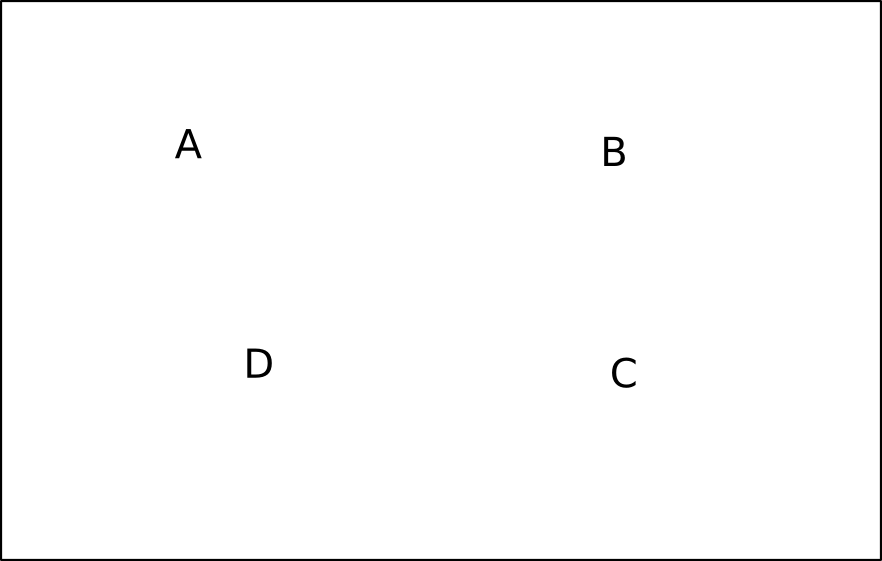
\includegraphics[scale=1.0]{"figures/michelson-morley.png"} \caption{Experimental layout of the Michelson-Morley type experiments}
\end{center}
\end{figure}

The interference pattern encodes the phase difference $ \Theta_1  - \Theta_2 $ between the Arahanov-Bohm phase changes experienced by the two beams as they travel between \textbf{A} and \textbf{C}, via the paths \textbf{ABC} and \textbf{AB'C} respectively.

Now let us assume that there exist fluxes, corresponding to the curvature $ F^I_{\mu\nu} $ of a gauge connection $ A^I_\mu $, piercing the surface bounded by the closed path \textbf{L${}_\gamma$} $ = $ \textbf{L\subsc{1}} $ \cup $ \textbf{L\subsc{2}}. Such a flux would take the form:

\begin{equation}\label{eqn:curvature_flux}
\delta \phi^I [ \mathcal{S} ] = \int_\mathcal{S} F^I_{\mu\nu} n^\mu dx^\nu 
\end{equation}

where $ I, J, K, \dots $ are Lie algebra indices, $ \mu, \nu, \dots $ are spacetime indices and $ \mathcal{S} $ denotes the surface bounded by \textbf{L${}_\gamma$}.

In the classic setup, the experimentalist employs light beams with the spin-1 photons being the corresponding excitations whose phase shifts are measured. However nothing prevents us from using any excitation we like from the particle spectrum of the standard model. Each excitation would undergo a phase shift corresponding to the flux of the connection associated with that particular excitation. For instance, electrons, muons and neutrinos would respond to the electroweak component of the flux while hadrons would respond to the strong component. If we were given some species of massless fermions which couple to the gauge group $ SU(2) $ for the gravitational connection, then their phases would measure the strength of the gravitational field in the region bounded by \textbf{L${}_\gamma$}.

For an abelian connection, such as a $ U(1) $ connection the Lie algebra is one-dimensional and its corresponding index is trivial. We have: $ F_{\mu\nu} = \partial_\mu A_\nu $, inserting this into \ref{eqn:curvature_flux} and using Stokes' theorem we find:

\begin{equation}\label{eqn:curvature_flux2}
\delta \phi [ \mathcal{S} ] = \int_\mathcal{S} \partial_\mu A_\nu n^\mu dx^\nu = \int_{L_\gamma} A(\vec{x}(\gamma))_\mu \cdot d\vec{x}(\gamma)^\mu
\end{equation}


For a non-abelian connection $ A^I_\mu $, the Lie-algebra index is non-trivial \emph{and} the expression for curvature has an additional term: $ F^I_{\mu\nu} = \partial_\mu A_\nu + g \, \epsilon^I_{JK} [ A^J_\mu, A^K_\nu ] $, where $ g $ determines the strength of the self-interactions of the gauge field. Consequently the expression for phase shift, or holonomy, becomes:

\begin{equation}\label{eqn:curvature_flux3}
\delta \phi^I [ \mathcal{S} ] = \int_\mathcal{S} \left\{ \partial_\mu A^I_\nu  + g \epsilon^I_{JK} [ A^J_\mu, A^K_\nu ] \right \} n^\mu dx^\nu = \int_{L_\gamma} A(\vec{x}(\gamma))_\mu \cdot d\vec{x}(\gamma)^\mu
	\end{equation}

\end{doublespace}






\chapter{BCS Gravity}

\begin{doublespace}

\section{Introduction}

Ever since the BCS theory of superconductivity has been discovered, the phenomenon of Cooper
pairing has played a seminal role across a wide range of physics, including Pion formation,
Technicolor and QCD at high densities.  A Cooper pair requires some necessary conditions:
\begin{itemize}
\item A Fermi surface. \item Screening resulting in an attractive interaction between fermions.
\item A relevant four-fermion interaction.
\end{itemize}

Another important aspect of the BCS theory is that it signifies that the perturbative vacuum with
respect to perturbative phonon or vector boson exchange is unstable; a very weak attractive
interaction drives the system to a lower energy non-perturbative ground state. In the context of
general relativity, graviton exchange between fermions is a ripe setting to ask whether or not a
BCS condensate can form. This possibility may have consequences, especially for the inflationary
paradigm and the cosmological constant problem since the idea that the vacuum is unstable with
respect to graviton exchange between fermions can pave a way to solving the cosmological constant
problem.  In this paper we demonstrate for the first time that gravity naturally incorporates a
BCS condensate in a %general, $\Lambda$ dominated,
FRW space-time. In the context of inflation this condensate can play the role of the inflaton
field. We show that the condensate behaves as a scalar field with a mass which is a montonically
decreasing function of the physical volume of the spatial hypersurfaces. The condensate mass is
large in the early universe when the spatial volume is very small and quantum correlations are
large. The scalar field sources inflation which lasts until its mass becomes negligible, at which
point only the kinetic term of the scalar field contributes and we enter a radiation like epoch
which slowly expanding scale factor and decaying hubble rate.

%We also show that the gap introduces a non-perturbative canceling
%correction to the cosmological constant which is consistent with the
%expectations of the authors as a possible path towards resolving the
%cosmological constant problem.

Recently \cite{Perez2006Physical} is was shown that gravity in the presence of a Dirac field induces
a non-zero torsion. This torsion turns out to be proportional to the axial current, $J_{\mu5}$.
Inserting the expression for the torsion back into the first-order action we find a new interaction
term which is proportional to the square of the axial current and also has a dependance on the
Immirzi parameter.\footnote{This four-fermion interaction is not new. As far back as 1922 Cartan
proposed that a correct theory of gravity should also contain torsion.} Such a four-fermi
interaction is well-known to cause the formation of a chiral condensate. As a consequence
$<\psi^\dag\psi>$ develops a non-zero vev and the resulting theory has a mass gap $\Delta$.

%We also find a negative contribution to the cosmological constant
%$\Lambda_0$ from the fermionic condensate.

The paper is arranged as follows. In Section 2 we show how the presence of a Dirac term in the
first-order action for fermions coupled to gravity, induces the four-fermion interaction. In
Section 3 we do the (3+1) decomposition of the resulting Lagrangian and find the Hamiltonian by
performing a Legendre transform. This allows us to identify the diffeomorphism, hamiltonian and
gauge constraints of the theory. It is the hamiltonian constraint which is responsible for dynamics
and we concentrate on it. In Section 4 we write down the hamiltonian constraint for a FRW metric.
We then quantize the fermion field, while leaving the background metric classical. In Section 5 we
exhibit the Boguliubov transformation on the fermionic ladder operators which is a necessary step
in the BCS calculation\footnote{The gap can also be determined via a variational method, however
the Boguliubov transformation is simpler and more instructive}. In Section 6 we diagonalize the
matter hamiltonian by applying the Boguliubov transformation and then find the gap equation. We
find that the matter part of the hamiltonian now behaves as a scalar field with mass $\Delta$,
decreases monotonically as the scale factor increases. We then discuss how this scalar field can
source an inflationary phase.

\section{Torsion and the four-fermi interaction}
Our starting point is with the Holst action for General Relativity with a cosmological constant,
coupled to fermions.  We will calculate the four-fermion interaction induced by Torsion and write
the action in Hamiltonian form.  The action will be symmetry reduced and after all of the
constraints are identified we will show that the fermionic Hamiltonian is a many-body BCS
Hamiltonian.  Finally we will diagonalize the Hamiltonian and calculate the energy gap.

First, it is convenient to introduce our conventions.  Lowercase greek letters $\mu,\nu,...$ stand
for four dimensional spacetime indices $1..4$. Lowercase latin letters denote spatial indices on
$\Sigma$. Uppercase latin $I,J,...$ denote internal indices $1..4$. Lowercase latin letters denote
internal indices $1..3$.

The action for gravity coupled with massless fermions is:

\begin{equation}\label{action}
    S[A,e,\Psi] = S_{H} + S_{D}
\end{equation}

where $S_{H}$ is the Holst action and is equivalent to the metric formulation of general
relativity:

\begin{equation}\label{holst_action}
    S_{H} = \frac{1}{2\kappa}\int d^{4}x\,e\,e^{\mu}_{I}e^{\nu}_{J}F^{IJ}_{\mu\nu} -
    \frac{1}{2\kappa\gamma}\int d^{4}x\,e\,e^{\mu}_{I}e^{\nu}_{J}\star F^{IJ}_{\mu\nu}
\end{equation}

and $S_{D}$ is the action for fermions:

\begin{equation}\label{dirac_action}
    S_{D} = \frac{i}{2}\int d^{4}x\,e\,(\bar{\Psi}\gamma^{I}e^{\mu}_{I}D_{\mu}\Psi -
    \overline{D_{\mu}\Psi}\gamma^{I}e^{\mu}_{I}\Psi)
\end{equation}

where:

\begin{eqnarray}\label{covariant_derivative}
    D_{\mu}\Psi = \partial_{\mu}\Psi - \frac{1}{4}A_{\mu}^{IJ}\gamma_{I}\gamma_{J}\Psi \\
    \overline{D_{\mu}\Psi} = \partial_{\mu}\bar{\Psi} + \frac{1}{4}\bar{\Psi}\gamma_{I}\gamma_{J}A_{\mu}^{IJ}
\end{eqnarray}

The equation of motion obtained by varying (\ref{action}) with respect to the four dimensional spin
connection $A_{\mu}^{IJ}$ yields:

\begin{equation}\label{connection}
    A_{\mu}^{IJ}=\omega_{\mu}^{IJ} + C_{\mu}^{IJ}
\end{equation}

where $\omega_{\mu}^{IJ}$ is the spin connection compatible with the tetrad $e_{I}^{\mu}$ and
$C_{\mu}^{IJ}$ is the tetrad projection of the contortion tensor:

\begin{equation}\label{contortion}
    C_{\mu}^{IJ} = C_{\mu}^{\nu\delta}e^{I}_{[\nu}e^{J}_{\delta]}
\end{equation}

On solving for $C_{\mu}^{IJ}$ in terms of the fermionic field and inserting the resulting
expression for $A_{\mu}^{IJ}$ in (\ref{action}) one obtains the following:

\begin{equation}\label{action2}
    S[e,\Psi] = \frac{1}{16\pi G}\int
    d^{4}x\,e\,e^{\mu}_{I}e^{\nu}_{J}F^{IJ}_{\mu\nu}[\omega(e)] + \frac{i}{2}\int d^{4}x\,e\,(\bar{\Psi}\gamma^{I}e^{\mu}_{I}D_{\mu}[\omega(e)]\Psi -
    \overline{D_{\mu}[\omega(e)]\Psi}\gamma^{I}e^{\mu}_{I}\Psi) +
    S_{int}[e,\Psi] + S_b
\end{equation}

where $S_{int}$ is the four fermion interaction\footnote{A detailed derivation is included in the
Appendix}:

\begin{equation}\label{int_action}
    S_{int} = -\frac{3}{2}\pi G \frac{\gamma^{2}}{\gamma^{2}+1}
    \int d^{4}x\,e (\bar{\Psi}\gamma_{5}\gamma_{I}\Psi)(\bar{\Psi}\gamma_{5}\gamma^{I}\Psi)
    = -\frac{3}{2}\pi G \frac{\gamma^{2}}{\gamma^{2}+1} \int d^{4}x\,e (j_a^I)^2
\end{equation}

and $S_b$ is a boundary term, given by:

\begin{equation}\label{boundary_term}
    S_b = -\frac{3}{4\kappa\gamma}\oint\limits_{\partial\Sigma}^{} d^3x n_\mu j_a^\mu
\end{equation}

Before we proceed to the $(3+1)$ decomposition of the above action, we write the Dirac action in
terms of Weyl spinors. This will make the decomposition simpler and will also illustrate an
important property of the left and right handed spinors \footnote{In the following we essentially
follow the Appendix of \cite{Thiemann1998Quantum}, filling in some of the steps. We have included this
derivation to make the paper self-contained.}

We expand the second term in (\ref{covariant_derivative})

\begin{eqnarray}\label{connection_decomp}
    A_\mu^{IJ}\gamma_I\gamma_J & = & A_\mu^{i0}\gamma_i\gamma_0 +
    A_\mu^{0i}\gamma_0\gamma_i + A_\mu^{ij} \gamma_i\gamma_j \nonumber \\
    & = & 2A_\mu^{0i}\gamma_0\gamma_i+ A_\mu^{ij}\gamma_i\gamma_j \nonumber  \\
    & = & 2A_\mu^{0i}\left(\begin{array}{cc}-\sigma_i&0\\0&\sigma_i\end{array}\right)
    + iA_\mu^{jk}\epsilon^{ijk}\left(\begin{array}{cc}\sigma_i&0\\0&\sigma_i\end{array}\right)\nonumber \\
    & = & 2i\left(\begin{array}{cc}A_\mu^{i+}\sigma_i&0\\0&A_\mu^{i-}\sigma_i\end{array}\right)
\end{eqnarray}

In the second line we have used the fact that $A_\mu^{IJ}$ is antisymmetric in the internal indices
and that the gamma matrices anticommute. In the third we have used the expressions for the gamma
matrices given in the appendix to expand out the matrix products. In the fourth we have used the
definition of the self and anti-self dual parts of the connection:

\begin{eqnarray}
    A_\mu^{i+} = \frac{1}{2}\epsilon^{ijk}A_\mu^{jk} + iA_\mu^{0i} \nonumber \\
    A_\mu^{i-} = \frac{1}{2}\epsilon^{ijk}A_\mu^{jk} - iA_\mu^{0i}
\end{eqnarray}

Now writing the Dirac spinor $\Psi$ in term of the Weyl spinors $\psi, \eta$, we see that
(\ref{covariant_derivative}) becomes:

\begin{equation}
    D_\mu\Psi = \left(\begin{array}{c}{\cal D}_\mu^+\psi\\{\cal D}_\mu^-\eta\end{array}\right)
\end{equation}

where ${\cal D}_\mu^+\psi=\partial_\mu\psi-\frac{i}{2}A_\mu^{i+}\sigma_i\psi$ and ${\cal
D}_\mu^-\eta=\partial_\mu\eta-\frac{i}{2}A_\mu^{i-}\sigma_i\eta$. Thus the left(right) handed
spinors couple to the self(anti-self) dual parts of the connection.

We now proceed with the (3+1) decomposition of (\ref{action2}).

\section{3+1 decomposition and Legendre Transform}

Consider a spacelike slice $\Sigma$ of the spacetime manifold ${\cal M}$ with unit normal
$n^{\mu}$. Then the Dirac action is:

\begin{eqnarray}\label{dirac_decomp}
    2S_{D} & = & i\int d^{3}x\,dt\,N\,\sqrt{q}\,
    (\bar{\Psi}\gamma_{\mu}{\cal D}_{\nu}\Psi - c.c.)(q^{\mu\nu}-n^{\mu}n^{\nu})\nonumber \\
    & = & i\int d^{3}x\,dt\,N\,\sqrt{q}
    (\bar{\Psi}\gamma^{a}{\cal D}_{a}\Psi + \bar{\Psi}\gamma^0n^{\nu}{\cal D}_{\nu}\Psi - c.c.)\nonumber \\
    & = & i\int d^{3}x\,dt\,N\,\sqrt{q}
    (\psi^\dag\sigma^{a}{\cal D}_{a}^{+}\psi - \eta^\dag\sigma^{a}{\cal D}_{a}^{-}\eta - c.c)
    +\sqrt{q}(t^{\mu}-N^{\mu})(\psi^\dag {\cal D}_{\mu}^{+}\psi + \eta^\dag {\cal D}_{\mu}^{-}\eta -
    c.c) \nonumber \\
    & = & i\int d^{3}x\,dt\,N\,\sqrt{q}
    (\psi^\dag\sigma^{a}{\cal D}_{a}^{+}\psi - \eta^\dag\sigma^{a}{\cal D}_{a}^{-}\eta - c.c) \nonumber \\
    &&+ \sqrt{q}(\psi^\dag\dot{\psi} + \eta^\dag\dot{\eta} -
    \frac{i}{2}A_t^{i\mathbb{C}}\psi^\dag\sigma_i\psi -
    \frac{i}{2}\bar{A}_t^{i\mathbb{C}}\eta^\dag\sigma_i\eta - c.c.) \nonumber \\
    &&- \sqrt{q}N^a(\psi^\dag {\cal D}_a^+\psi + \eta^\dag {\cal D}_a^-\eta - c.c.)
\end{eqnarray}

In the first line we have used the decomposition of the metric $g_{\mu\nu}$ on ${\cal M}$ in terms
on the metric $q_{ab}$ on $\Sigma$ and the unit normal $n^{\mu}$ to $\Sigma$. $q^{\mu\nu}$ projects
tensors and derivatives on ${\cal M}$ to tensors and derivatives on $\Sigma$. ${\cal D}_{\mu}$ and
${\cal D}_{a}$ denote the covariant derivative on ${\cal M}$ and its restriction to $\Sigma$
respectively. In the second line we have used the freedom to fix the gauge in the internal space
such that the contraction of $\gamma_{\mu}$ and $n^{\mu}$ gives us $-\gamma^{0}$. In the third the
decomposition of $n^{\mu}$ in terms of the timelike vector field $t^{\mu}$, the lapse $N$ and the
shift $N^{\mu}$, and the expression of the covariant derivative in terms of the self and anti-self
dual parts of the connection is used. In the last line we have noted that the restriction of
$A_\mu^{i+}$ to $\Sigma$ is the Ashtekar connection $\Gamma_a^i + iK_a^i$. The time component of
$A_\mu^{i+}$ is written as $A_t^{i\mathbb{C}}$.

Using $A_t^j = \tt{Re}(A_t^{j\mathbb{C}})$ and evaluating the complex conjugate terms explicitly we
get:

\begin{eqnarray}\label{dirac_decomp2}
    S_D & = &  \frac{i}{2}\int d^{3}x\,dt \sqrt{q}(\psi^\dag\dot{\psi} +
    \eta^\dag\dot{\eta} - c.c.) - i\sqrt{q} A_t^{i}(\psi^\dag\sigma_i\psi + \eta^\dag\sigma_i\eta) \nonumber \\
    && - \sqrt{q}N^a(\psi^\dag D_a\psi + \eta^\dag D_a\eta - c.c.) \nonumber \\
    && + N\left[E^a_i(\psi^\dag\sigma^i D_a\psi - \eta^\dag\sigma^i D_a\eta - c.c.)
    + i[K_a,E^a]^k(\psi^\dag\sigma_k\psi + \eta^\dag\sigma_k\eta) \right]
\end{eqnarray}

Here $D_a\psi = \partial_a\psi - \frac{i}{2}\Gamma_a^i\sigma_i\psi$. We can easily see that
contributions of the Dirac action to the gauss, scalar and diffeomorphism constraints are the
coefficients of $A^i_t$, $N$ and $N^a$ respectively. The decomposition of $S_{int}$ is easily done
and we obtain the following form:

\begin{eqnarray}\label{interaction_decomp}
    S_{int} & = &  -\frac{3}{2}\pi G \frac{\gamma^{2}}{\gamma^{2}+1}
                    \int d^{3}x\,dt \sqrt{q}N\left[(\psi^\dag\sigma^a\psi + \eta^\dag\sigma^a\eta)^2 - (-\psi^\dag\psi +
                    \eta^\dag\eta)^2\right]
\end{eqnarray}

From (\ref{dirac_decomp2}) we see that Lagrange multiplier of the matter contribution to the
gravitational gauss constraint is $\tt{Re}(A^{i\mathbb{C}}_t)$. In order to get this Lagrange
multiplier one must first start with the 3+1 decomposition of the self-dual gravitational action
and then take its real part. The self-dual gravitational action is:

\begin{equation}\label{self-dual_action}
    S_{SD} = \frac{1}{\kappa}\int d^4x\,e^a_I e^b_J {}^{+}F_{ab}^{IJ}
\end{equation}

${}^{+}F_{ab}^IJ$ is the curvature of the self-dual connection and $e^a_I$ is the usual tetrad.
Doing the 3+1 decomposition in the usual manner yields:

\begin{equation}\label{self-dual_decomp}
    S_{SD} = \frac{1}{\kappa}\int d^3x\,dt\, \left[-i \tilde{E}^b_i\dot{A}_b^i -
    i A_t^{i\mathbb{C}} {\cal D}_b(\tilde{E}^b_i) - i N^a
    tr[F_{ab}\tilde{E}^b] +
    \frac{N}{2\sqrt{q}}tr(F_{ab}[\tilde{E}^a,\tilde{E}^b])\right]
\end{equation}

where $\tilde{E}^b_i$ is the densitized triad, $F_{ab}^i$ is the curvature of the restriction
$A_b^i$ to $\Sigma$ of the complex self-dual connection, and the trace and commutators are taken in
the Lie-algebra of su(2).

Taking the real part of the above action and using the fact that $A_a^i = \Gamma_a^i + iK_a^i$ we
get:

\begin{equation}\label{real_gravitational_action}
    S_{real} = \frac{1}{\kappa}\int
    d^3x\,dt\,\left\{\tilde{E}^b_i \dot{K}^i_b + A^i_t[K_b,\tilde{E}^b]^i
    + 2 N^a D_{[a}K_{b]}^i\tilde{E}^b_i \\
    + \frac{N}{2\sqrt{q}}(R_{ab}^i -[K_a,K_b]^i)[\tilde{E}^a,\tilde{E}^b]_i
    \right\}
\end{equation}

From (\ref{dirac_decomp2}) we see that the momenta conjugate to $\psi$ and $\psi^\dag$ are
$\frac{i}{2}\psi^\dag$ and $-\frac{i}{2}\psi$ respectively.. Then doing the Legendre transform on
$S_{real} + S_D + S_{int}$ we get the following Hamiltonian:

\begin{eqnarray}\label{total_hamiltonian}
    \lefteqn{H_{G+D+int}  =  \int d^{3}x\, A_t^{i}\left\{\frac{1}{\kappa}[K_b,\tilde{E}^b]^i + j^i \right\}}\nonumber \\
     & &{}+N\bigg\{\frac{1}{2\kappa\sqrt{q}}(R_{ab}^i-[K_a,K_b]^i)[\tilde{E}^a,\tilde{E}^b]_i
     +\frac{i}{2\sqrt{q}}\tilde{E}^a_i(\xi^\dag\sigma^i D_a\xi - \rho^\dag\sigma^i D_a\rho - c.c.)\nonumber \\
     & &{}+\frac{1}{2}[K_a,\tilde{E}^a]^k j_k
     - \frac{3}{2} \pi G \frac{\gamma^{2}}{\gamma^{2}+1}[j^2 - (-\xi^\dag\xi + \rho^\dag\rho)^2] + \sqrt{q}\Lambda_0\bigg\} \nonumber \\
     & &{}+N^a\left\{\frac{2}{\kappa}D_{[a}K_{b]}^i\tilde{E}^b_i +
    \frac{i}{2}(\xi^\dag D_a\xi + \rho^\dag D_a\rho - c.c.)\right\}
\end{eqnarray}

where $\xi=q^\frac{1}{4}\psi; \rho=q^\frac{1}{4}\eta$ and $j^i = (\eta^\dag\sigma^i\eta +
\rho^\dag\sigma^i\rho)/2$ is the axial current . We must change variables to make the matter fields
half-densities, because otherwise the connection would become complex \cite{Thiemann1998Quantum}. The
hamiltonian is manifestly a sum of constraints and the form of each constraint is easy to read off
from (\ref{total_hamiltonian}). It is important to note the gravitational Gauss constraint now has
a matter contribution. In the third line we have also added a term coming from the bare
cosmological constant.

\section{Symmetry Reduction and quantization}

We make the ansatz that the background metric is FRW with scale factor $a$. The basic gravitational
variables are:

\begin{eqnarray}\label{FRWMetricVariables}
    E_i^a = a^2\delta^a_i & K_a^i = a^2\dot{a}\delta^a_i & R_{ab}^i = 0
\end{eqnarray}

We assume, for the moment, that the axial current is zero and hence the Gauss constraint is
satisfied. We also assume that the matter contribution to the diffeomorphism constraint is zero.
Later we shall find that these statements are true when we quantize the fermionic field. We are
left with the hamiltonian constraint and this reduces to:

\begin{equation}\label{ReducedHamiltonian}
    {\cal H} = {\cal H}_G + {\cal H}_D + {\cal H}_{int}= -\frac{3}{\kappa}a^3H^2 + a^3\Lambda_0 +
    \frac{i}{a}\left(\xi^\dag\sigma^a\partial_a\xi - \rho^\dag\sigma^a\partial_a\rho\right)
    + \frac{3\kappa}{32a^3}\frac{\gamma^2}{\gamma^2+1}\left[\xi^\dag\xi - \rho^\dag\rho\right]^2 = 0
\end{equation}

where $H = (\dot{a}/a)$ is the Hubble parameter.

We switch to physical co-ordinates in order to take care of the factor of $1/a$ in ${\cal H}_D$.
${\cal H}_D$ reduces to $i(\xi^\dag\sigma^a\partial_a\xi - \rho^\dag\sigma^a\partial_a\rho)$. We
can then expand $\xi$ and $\rho$ in terms of fourier modes:

\begin{subequations}\label{FermionFourierModes}
\begin{equation}
    \xi(x) = \int \frac{d^3k}{(2\pi)^3} \left\{ \xi_{k\uparrow}e^{-ikx} + \xi_{k\downarrow}e^{-ikx} \right\}
\end{equation}
\begin{equation}
    \rho(x) = \int \frac{d^3k}{(2\pi)^3} \left\{ \xi_{k\downarrow}e^{-ikx} + \xi_{k\uparrow}e^{-ikx} \right\}
\end{equation}
\end{subequations}

where $\xi_{k\uparrow}$ ($\xi_{k\downarrow}$) is a spinor\footnote{The expressions for these
spinors are given in the Appendix} of density weight $1/2$ \footnote{Because as mentioned earlier
the fermionic fields must be half-densities} along the direction $\hat{k}$ in momentum space and
with spin up (down) along $\hat{k}$, and corresponding to eigenvalue $+|k|$ ($-|k|$). The positive
(negative) helicity modes correspond to positive (negative) frequencies for $\xi$ and vice versa
for $\rho$. Thus we can write the quantized field in the usual manner in term of anticommuting
annihilation and creation operators:

\begin{subequations}\label{QuantizedFermionField}
\begin{equation}
    \hat\xi(x) = \int \frac{d^3k}{(2\pi)^3} \left\{ a_k \xi_{k\uparrow} + b^\dag_{-k} \xi_{k\downarrow} \right\} e^{-ikx}
\end{equation}
\begin{equation}
    \hat\rho(x) = \int \frac{d^3k}{(2\pi)^3} \left\{ \bar b_k \xi_{k\downarrow} + \bar a^\dag_{-k} \xi_{k\uparrow} \right\}e^{-ikx}
\end{equation}
\end{subequations}

$\rho$ and $\xi$ are independent fields, therefore we have used $\bar{}$ to distinguish their
operators. These fields satisfy the anticommutation relations:

\begin{subequations}\label{Anticommutation}
\begin{equation}
    \{\hat\xi^\dag_\alpha(x),\hat\xi_\beta(y)\} = \{\hat\rho^\dag_\alpha(x),\hat\rho_\beta(y)\} =
    (2\pi)^3\delta_{\alpha\beta}\delta^3(x,y)\sqrt{q}
\end{equation}
\begin{equation}
    \{\hat\xi_\alpha(x),\hat\xi_\beta(y)\} = \{\hat\xi^\dag_\alpha(x),\hat\rho_\beta(y)\} = 0
\end{equation}
\end{subequations}


The above expressions for the quantized field can be used to easily verify that the spatial current
and the matter contribution to the diffeomorphism constraint are zero, as stated previously. Using
the orthogonality of spinors of opposite helicity, the quantized form of the free Dirac hamiltonian
is easily found to be:

\begin{equation}\label{QuantizedDiracHam}
    \hat{\cal H}_D = \hat{\cal H}_\xi + \hat{\cal H}_\rho = \int \frac{d^3k}{(2\pi)^3}\,|k|
            (a^\dag_k a_k + b^\dag_{-k} b_{-k} + \bar a^\dag_{-k} \bar a_{-k} + \bar b^\dag_k \bar b_k)
\end{equation}

\section{Boguliubov transformation}

The four-fermi interaction is identical to the one which describes the formation of a condensate in
BCS theory \cite{Fetter2003Quantum}. Due to this interaction the true vacuum is not the one
corresponding to the Dirac equation but one in which particles and antiparticles of opposite
momenta and helicity are paired\footnote{In BCS theory the pairing happens between particles of
opposite momenta. However, here we have left and right handed fermions therefore the pairing must
include the helicity}. The interacting part is non-diagonal in the present variables. In order to
diagonalize the full matter hamiltonian we have to perform a Boguliubov transformation, which is a
linear canonical transformation to new annihilation and creation operators. We get a new ground
state corresponding to these operators. This BCS ground state is a condensate of Cooper pairs.
Excitations of this "vacuum" are produced by the action of the new operators whose physical effect
is to break up Cooper pairs and produce free fermions and antifermions.

\begin{subequations}\label{BogTrans}
\begin{equation}
    \alpha_k = u_k a_k - v_k b^\dag_{-k}
\end{equation}
\begin{equation}
    \beta_{-k} = u_k b_{-k} + v_k a^\dag_k
\end{equation}
\end{subequations}

Then the new variables $\alpha_k$ and $\beta_{-k}$ satisfy anticommutation relations if $u_k^2 +
v_k^2 = 1$. In terms of the new variables, the old ones are:

\begin{subequations}\label{InverseBogTrans}
\begin{equation}
    a_k = u_k \alpha_k + v_k \beta^\dag_{-k} \\
\end{equation}
\begin{equation}
    b_{-k} = u_k \beta_{-k} - v_k \alpha^\dag_k
\end{equation}
\end{subequations}

In the new variables $\hat{\cal H}_\xi$ becomes:

\begin{equation}\label{FreeTerm}
    \hat{\cal H}_\xi = \int \frac{d^3k}{(2\pi)^3}\, |k| \left(2v_k^2  + (u_k^2 - v_k^2)(m_k + n_{-k}) + 2u_k v_k\Sigma_k\right)
\end{equation}

where $m_k = \alpha^\dag_k\alpha_k$ , $n_{-k} = \beta^\dag_{-k}\beta_{-k}$ are the new number
operators and $\Sigma_k = \alpha^\dag_k\beta^\dag_{-k} + \beta_{-k}\alpha_k$ is the off-diagonal
part.

\section{Four-fermion term}

The interaction hamiltonian is an attractive four-fermion term which causes the formation of the
fermion condensate. In the this section we use the mode expansion for the fermion field to expand
this term and then apply the Boguliubov transformation to it.

The four-fermion term is:

\begin{eqnarray}\label{FourFermionTerm}
    \hat H_{int} &=& \frac{3\kappa}{32a^3}\frac{\gamma^2}{\gamma^2+1}
            \int d^3x\,\left(\hat\xi^\dag\hat\xi - \hat\rho^\dag\hat\rho\right)^2 \nonumber \\
    &=&  \frac{\alpha}{a^3} \int d^3x\, \left(\hat\xi^\dag\hat\xi\hat\xi^\dag\hat\xi +
                \hat\rho^\dag\hat\rho\hat\rho^\dag\hat\rho
                - \hat\rho^\dag\hat\rho\hat\xi^\dag\hat\xi - \hat\xi^\dag\hat\xi\hat\rho^\dag\hat\rho
                \right) \nonumber \\
    &=& \hat H_1 + \hat H_2 + \hat H_{\rho\xi} + \hat H_{\xi\rho}
\end{eqnarray}

where $\alpha = \frac{3\kappa}{32}\frac{\gamma^2}{\gamma^2+1}$. Now we can write $\hat\rho$ as:

\begin{equation}\label{rho}
    \hat\rho(x) = \int \frac{d^3k}{(2\pi)^3} \left\{\bar b_{-k} \xi_{k\uparrow}+\bar a^\dag_{k} \xi_{k\downarrow}\right\}e^{ikx}
\end{equation}

by doing changing variables from $k$ to $-k$ in the integration. Then by comparing (\ref{rho}) and
(\ref{QuantizedFermionField}a) we see that one can switch from $\hat\xi$ to $\hat\rho$ (or vice
versa) by changing $a_k \leftrightarrow \bar b_{-k}$.

Now using the anticommutation relations for the fermionic fields we can write $\hat H_1$ as:

\begin{equation}
    \hat H_1 = \alpha \int d^3x\, \hat\xi^\dag \hat\xi -
    \frac{\alpha}{a^3} \int d^3x\,
    \hat\xi^\dag_\alpha\hat\xi^\dag_\beta\hat\xi^\beta\hat\xi^\alpha
    = \hat N_\xi + \hat H_{\xi\xi}
\end{equation}

Using (\ref{QuantizedFermionField}a) and (\ref{BogTrans}) $\hat N_\xi$ becomes:

\begin{equation}\label{xiNumberOp}
    \hat N_\xi = \alpha \int \frac{d^3k}{(2\pi)^3}\, \left[a^\dag_k a_k - b^\dag_{-k} b_{-k} \right]
                = \alpha \int \frac{d^3k}{(2\pi)^3}\, \left[m_k - n_{-k} \right]
\end{equation}

Likewise for $\hat\rho$ we have:

\begin{equation}
    \hat H_2 = \alpha \int d^3x\, \hat\rho^\dag\rho -
    \frac{\alpha}{a^3} \int d^3x\,
    \hat\rho^\dag_\alpha\hat\rho^\dag_\beta\hat\rho^\beta\hat\rho^\alpha
    = \hat N_\rho + \hat H_{\rho\rho}
\end{equation}

and $\hat N_\rho$ is:

\begin{equation}\label{rhoNumberOp}
    \hat N_\rho = \alpha \int \frac{d^3k}{(2\pi)^3}\, \left[\bar b^\dag_k \bar b_k - \bar a^\dag_{-k} \bar a_{-k} \right]
                = \alpha \int \frac{d^3k}{(2\pi)^3}\, \left[\bar n_k - \bar m_{-k} \right]
\end{equation}

To explicitly evaluate $\hat H_{\xi\xi}$ and $\hat H_{\rho\xi}$ we use the mode expansion
(\ref{QuantizedFermionField}) and the anticommutation relations of the fermionic operators. Then
$\hat H_{\rho\rho}$ and $\hat H_{\xi\rho}$ are obtained by simply using the substitution $ a_k
\leftrightarrow b_{-k}$. After some algebra we obtain the following expression:

\begin{multline}\label{InteractionTerm}
    \hat H_{\xi} + \hat H_{\xi\xi} + \hat N_{\xi} =
    \int \frac{d^3k}{(2\pi)^3} |k|(a^\dag_k a_k + b^\dag_{-k} b_{-k}) -
    \alpha  \int \frac{d^3k d^3p}{(2\pi)^6}\,
    2 a^\dag_k a_k \left[
    \left(\xi^\dag_{k\uparrow}\xi_{p\downarrow}\right)\left(\xi^\dag_{p\downarrow}\xi_{k\uparrow}\right)
    +{}1 \right] \\
    -{}\alpha  \int \frac{d^3k d^3p d^3k'd^3p'}{(2\pi)^6}\, \delta^3(k+k'-p-p')
    \bigg\{
    a^\dag_k a^\dag_{k'} a_p a_{p'}\left(\xi^\dag_{k\uparrow}\xi_{p\uparrow}\right)\left(\xi^\dag_{k'\uparrow}\xi_{p'\uparrow}\right)
    + \\
    b^\dag_{-k} b^\dag_{-k'} b_{-p} b_{-p'} \left(\xi^\dag_{p\downarrow}\xi_{k\downarrow}\right)\left(\xi^\dag_{p'\downarrow}\xi_{k'\downarrow}\right)
    \bigg\} + \delta^3(k-k'+p-p')
    a^\dag_k b^\dag_{-k'} b_{-p} a_{p'} \bigg\{
    \left(\xi^\dag_{k\uparrow}\xi_{k'\downarrow}\right)\left(\xi^\dag_{p\downarrow}\xi_{p'\uparrow}\right)
    \\
    + \left(\xi^\dag_{k\uparrow}\xi_{p'\uparrow}\right)\left(\xi^\dag_{p\downarrow}\xi_{k'\downarrow}\right)
    \bigg\} + \alpha  \int \frac{d^3k}{(2\pi)^3}\, \left[a^\dag_k a_k - b^\dag_{-k} b_{-k} \right]\\
    = \hat H_{\xi} + \alpha  \int \frac{d^3k d^3p}{(2\pi)^6}\, A_0 V_0
    -\alpha  \int \frac{d^3k d^3p d^3k'd^3p'}{(2\pi)^6}\, \big[\delta^3(k+k'-p-p')(A_1 V_1 + A_2 V_2) +  \\
    \delta^3(k-k'+p-p') A_3 V_3 \big] + \hat N_{\xi}
\end{multline}

In the last line the $A${\small s} denote the operator products and the $V${\small s} denote the
spinor products. Also in the above expression and henceforth we only use dedensitized spinors.
There is a factor of $a^3$ in front of the whole expression which we set to $1$ for now. The factor
is re-introduced later when appropriate.

Now using momentum conservation we can simplify $A_1$ as follows.

\begin{equation}
    A_{1} = a^\dag_k a^\dag_{k'} a_p a_{p'} = a^\dag_k a^\dag_{k'} a_{k-q} a_{k'+q}
\end{equation}

Using Wick's theorem and the operator identities in the Appendix the above expression can be
written as:

\begin{eqnarray}\label{NormalOrderedOps}
    A_{1} &=& N(A_{1})+ \bigg\{ - N(a^\dag_k a_{k-q})\wick{1}{<1a^\dag_{k'}>1a_{k'+q}}
    - N(a^\dag_{k'} a_{k'+q})\wick{1}{<1a^\dag_{k}>1a_{k-q}}
    + N(a_k^\dag a_{k'+q}) \wick{1}{<1a^\dag_{k'}>1a_{k-q}} \nonumber \\
    &&{} +N(a_{k'}^\dag a_{k-q})\wick{1}{<1a^\dag_{k}>1a_{k'+q}}
    - \wick{1}{<1a^\dag_{k}>1a_{k-q}} \wick{1}{<1a^\dag_{k'}>1a_{k'+q}}
    + \wick{1}{<1a^\dag_{k}>1a_{k'+q}} \wick{1}{<1a^\dag_{k'}>1a_{k-q}} \bigg\}\nonumber \\
    &=&N(A_{1}) +\bigg\{- N(a^\dag_k a_k) v^2_{k'} \delta_{q,0} - N(a^\dag_{k'} a_{k'}) v^2_k \delta_{q,0}
            + N(a^\dag_k a_k) v^2_{k'}\delta_{k',k-q} + \nonumber \\
         &&   N(a^\dag_{k'} a_{k'}) v^2_k\delta_{k',k-q} - v^2_k v^2_{k'} \delta_{q,0} + v^2_k v^2_{k'} \delta_{k',k-q}
            \bigg\}
\end{eqnarray}

Inserting the above expression for $A_1$ into (\ref{InteractionTerm}) and integrating first over
the delta function in (\ref{InteractionTerm}) and then over the delta functions in
(\ref{NormalOrderedOps}) we obtain after relabelling some indices and some algebraic manipulations
we have:

\begin{multline}\label{Int1}
  - \alpha  \int \frac{d^3k d^3k' d^3q}{(2\pi)^9}\, A_1 V_1(k,k',q)
            = \\-N(V_1) + \alpha  \int \frac{d^3k d^3k'}{(2\pi)^6}\,
    \left[ N(a^\dag_k a_k)v^2_{k'} + N(a^\dag_{k'}a_{k'})v^2_k + v^2_k v_{k'}^2 \right]
    \left[ 1 -
    \left(\xi^\dag_{k\uparrow}\xi_{k'\uparrow}\right)\left(\xi^\dag_{k'\uparrow}\xi_{k\uparrow}\right)
    \right]
\end{multline}

where $N(V_1)$ is quartic in the creation and annihilation operators.

$A_2$ can be dealt with in a similar manner and after some computations we find:

\begin{multline}\label{Int2}
    - \alpha  \int \frac{d^3k d^3k' d^3q}{(2\pi)^9}\, (A_1 V_1 + A_2 V_2) = \\
    -N(V_1 + V_2) - \alpha  \int \frac{d^3k d^3k'}{(2\pi)^6}\, 2
    \left[N(a^\dag_k a_k) + N(b^\dag_{-k}b_{-k}) + v^2_k \right] v^2_{k'}
    \left[
    \left(\xi^\dag_{k\uparrow}\xi_{k'\uparrow}\right)\left(\xi^\dag_{k'\uparrow}\xi_{k\uparrow}\right)
    -1
    \right]
\end{multline}

The term with $A_3$ yields:

\begin{multline}\label{Int3}
    - \alpha  \int \frac{d^3k d^3k' d^3q}{(2\pi)^9}\, A_3 V_3 =
    - N(V_3) - \bigg \{
    \left[N(a^\dag_k a_k) + N(b^\dag_{-k}b_{-k}) + v^2_k \right]v^2_{k'}
    \left[
    \left(\xi^\dag_{k\uparrow}\xi_{k'\downarrow}\right)\left(\xi^\dag_{k'\downarrow}\xi_{k\uparrow}\right) + 1
    \right] \\
    + \left[N(a^\dag_k b^\dag_{-k}) + N(b_{-k}a_k) + u_k v_k \right]u_{k'}v_{k'}
    \Re \left[ \left(\xi^\dag_{k\uparrow}\xi_{k'\uparrow}\right)\left(\xi^\dag_{k'\downarrow}\xi_{k\downarrow}\right)
    \right] \bigg\}
\end{multline}

Above we have dealt with the terms of $\hat H_{\xi\xi}$. Doing similar manipulations with $\hat
H_{\xi\rho}$ we find:

\begin{equation}\label{IntCross}
    \hat H_{\xi\rho} = \hat H_{\rho\xi} = - \alpha  \int \frac{d^3k d^3k'}{(2\pi)^6}\,
    \left( a^\dag_k a_k - b^\dag_{-k} b_{-k} + \bar b^\dag_{-k} \bar b_{-k} - \bar a^\dag_k \bar a_k \right)
\end{equation}

In the above equation we have a seemingly divergent integral over the momenta $k'$. This is dealt
with by imposing a momentum cutoff. We get:

\begin{equation*}
    \int \frac{d^3k}{2\pi^3} = \frac{1}{2\pi^2}\int k^2 dk
    = \frac{1}{2\pi^2}\int\limits_{0}^{\hbar \omega_D} E^2 dE =
    \frac{(\hbar\omega_D)^3}{6\pi^2}=C_1
\end{equation*}

The sum of (\ref{FreeTerm}), (\ref{Int1}), (\ref{Int2}), (\ref{Int3}) and the first half of
(\ref{IntCross}) gives us the matter hamiltonian corresponding only to the field $\xi$. The other
half corresponding to $\rho$ can be is identical except for the substitution $a_k \leftrightarrow
\bar b_{-k}$.

\begin{multline}
    \hat H(\xi) =  \int \frac{d^3k}{(2\pi)^3} \left( a^\dag_k a_k + b^\dag_{-k} b_{-k}\right) \left( |k| - C_1\alpha \right)
        - \alpha  \int \frac{d^3k}{(2\pi)^3}\bigg\{ \left[ N(a^\dag_k b^\dag_{-k}) + N(b_{-k} a_k) + u_k v_k \right] u_{k'} v_{k'} V'_1  \\
        + \left[ N(a^\dag_k a_k) + N(b^\dag_{-k} b_{-k}) + v^2_k \right] v^2_{k'} V'_2 \bigg\} \\
        =  \int \frac{d^3k}{(2\pi)^3} \left[ (u^2_k - v^2_k)(m_k + n_{-k}) + 2 u_k v_k \Sigma_k + 2v^2_k \right](|k|- C_1\alpha)
         - \alpha  \int \frac{d^3k d^3k'}{(2\pi)^6} \bigg\{ \big[(u^2_k - v^2_k)\Sigma_k \\
         + 2 u_k v_k (m_k + n_{-k}) + u_k v_k \big] u_{k'} v_{k'}V'_1
        + \left[ (u^2_k - v^2_k)(m_k + n_{-k}) + 2 u_k v_k \Sigma_k + v^2_k \right] v^2_{k'} V'_2
        \bigg\}
\end{multline}

where:

\begin{subequations}
\begin{equation}
    V'_1(k,k') = \mathbb{Re}\left\{(\xi^\dag_{k\uparrow}\xi_{k'\uparrow})(\xi^\dag_{k'\downarrow}\xi_{k\downarrow}) \right\}
\end{equation}
\begin{equation}
    V'_2(k,k') = (\xi^\dag_{k\uparrow}\xi_{k'\uparrow})(\xi^\dag_{k'\uparrow}\xi_{k\uparrow}) +
            (\xi^\dag_{k\uparrow}\xi_{k'\downarrow})(\xi^\dag_{k'\downarrow}\xi_{k\uparrow}) = 1
\end{equation}
\end{subequations}

Where in the second line we have used the expressions for spinors given in the Appendix. Now we can
easily apply the Boguliubov transformation to the above hamiltonian and then collect terms
according to their operator coefficients. This process yields:

\begin{multline}\label{FullMatterHam}
    \hat H(\xi) = -\hat N(V) +  \int\frac{d^3k}{(2\pi)^3} \bigg\{ (m_k + n_{-k})\left[ (u^2_k - v^2_k)E_k + 2u_k v_k \Delta_k
    \right] + \Sigma_k \left[ 2u_k v_k E_k - (u^2_k - v^2_k)\Delta_k \right] \\
    + \left[ 2v^2_k E_k + E'v^2_k - u_k v_k \Delta_k \right] \bigg\}
     = -\hat N(V) + \hat K_1 + \hat K_2 + \hat U
\end{multline}

where:

\begin{subequations}\label{Defs}
\begin{equation}
    E' = \alpha \int \frac{d^3k'}{(2\pi)^3} \frac{v_{k'}^2}{2} V'_2(k,k')
\end{equation}
\begin{equation}
    E_k =  |k| - C_1\alpha - E'
\end{equation}
\begin{equation}
    \Delta_k = \alpha \int \frac{d^3k'}{(2\pi)^3} V'_1(k,k') u_{k'} v_{k'}
\end{equation}
\end{subequations}

In order to make the full matter hamiltonian diagonal we set the coefficient of $\Sigma_k$ in
(\ref{FullMatterHam}) to zero. This allows us to solve for $u_k$ and $v_k$ in terms of $\Delta_k$
and $E_k$.

Since $u_k^2 + v_k^2=1$, it is natural to use trigonometric variables. We set $u_k = \cos\theta$
and $v_k = \sin\theta$. Then we have:

\begin{eqnarray}\label{GapEqn1}
    &&2 u_k v_k E_k - (u_k^2 - v_k^2)\Delta_k = 0 \\
    \Rightarrow && \sin(2\theta) E_k = \cos(2\theta) \Delta_k \nonumber \\
    \Rightarrow && \tan(2\theta) = \frac{\Delta_k}{E_k}, \quad
    \sin(2\theta) = \frac{\Delta_k}{\sqrt{\Delta^2_k + E^2_k}} = \frac{\Delta_k}{\epsilon_k}, \quad
    \cos(2\theta) = \frac{E_k}{\epsilon_k}
\end{eqnarray}

Using the above the various terms in (\ref{FullMatterHam}) become:

\begin{subequations}\label{FinalMatterHam}
 \begin{equation}\label{PotentialEnergy}
   \hat U =  \int \frac{d^3k}{(2\pi)^3} \left\{ \left(1 - \frac{E_k}{\epsilon_k}\right)\left(E_k + \frac{E'_k}{2}\right) - \frac{\Delta_k^2}{2 \epsilon_k}  \right\}
\end{equation}
\begin{equation}
    \hat K_1 =  \int \frac{d^3k}{(2\pi)^3} \epsilon_k(m_k + n_{-k})
\end{equation}
\end{subequations}

From (\ref{FinalMatterHam}b) it is clear that the spectrum is now bounded from below by $\Delta_k$
which therefore is the mass gap.

%Now we do a rough calculation to estimate the value of $\Delta_k$. First let:

Now we make a change of variables in order to find the gap equation. Let:

\begin{equation}
    u_k = (\frac{1}{2} + x_k)^\frac{1}{2} \quad v_k = (\frac{1}{2} - x_k)^\frac{1}{2}
\end{equation}

Then (\ref{GapEqn1}) becomes:

\begin{eqnarray}
    && 2 u_k v_k E_k - (u_k^2 - v_k^2)\Delta_k = 0 \nonumber \\
    \Rightarrow && 2E_k(\frac{1}{4} - x_k^2)^\frac{1}{2} - 2x_k \Delta_k \nonumber \\
    \Rightarrow && x_k = \pm\frac{E_k}{2\sqrt{E_k^2 + \Delta_k^2}} \nonumber \\
 \end{eqnarray}

Inserting the solution for $x_k$ into the expression (\ref{Defs}c) for $\Delta_k$, we get the gap
equation:

\begin{equation}\label{GapEqn2}
    \Delta_k = \alpha \int \frac{d^3k'}{(2\pi)^3} \frac{V'_1(k,k')\Delta_{k'}}{2\sqrt{E_{k'}^2 + \Delta_{k'}^2}}
\end{equation}

In the above expression the potential  $ V'_1 \sim \mathcal{O}(1)$. We use a mean-field
approximation to set the value of this potential to a constant $V_a$. Then it is also consistent to
assume that $\Delta_k \equiv \Delta \, \forall \, k$.

Now we quantize our fermions in a box of size $L$. Then we have the following relation between the
density of states and the volume in momentum-space:

\begin{equation}\label{DOS}
    D(E)dE = \frac{4 \pi k^2 dk}{(\pi/L)^3}
\end{equation}

Then (\ref{GapEqn2}) becomes:

\begin{eqnarray}\label{GapEqn3}
    && \Delta = \frac{ \pi^3 \alpha V_a}{L^3} \int dE \, D(E) \frac{\Delta}{2\sqrt{E_k^2 +
    \Delta^2}} \nonumber \\
    \Rightarrow && 1 \approx \frac{\pi^3 \alpha V_a D(0)}{L^3} \int\limits_{-\hbar\omega_D}^{\hbar\omega_D} dE \frac{\Delta}{2\sqrt{E^2 +
    \Delta^2}} \nonumber \\
    \Rightarrow && 1 \approx \frac{\pi^3 \alpha V_a D(0)}{2L^3}
    \ln\frac{\sqrt{(\hbar\omega_D)^2 + \Delta^2} + \hbar\omega_D}{\sqrt{(\hbar\omega_D)^2 + \Delta^2} - \hbar\omega_D} \nonumber \\
    \Rightarrow && \Delta \approx \frac{2\hbar\omega_D }{sinh(\nu/2)} \qquad \left(\nu = \frac{2 L^3}{\pi^3 \alpha V_a D(0)} \right)
\end{eqnarray}

In the second line we have restricted our range of integration over the energy to a small region of
width $2\hbar \omega_D$ around the fermi surface. This is the only region in momentum space where
electrons are free to have interactions. We take the density of states in the interaction region to
be a constant $D(0)$ equal to the density of states at the fermi surface.

%where in the first line we have used the fact that $\frac{d^3k}{2\pi^3} \approx D(0) dE_k$. $D(0)$ is the density of
%states at the fermi surface. Now the density of states, $D(E)$, for a field in a 3-dimensional box of volume $V$ is:
%
%\begin{equation}
%     D(E) = \frac{d\,N}{d\,E} = \frac{d\,N}{d\,K}\frac{d\,K}{d\,E} = \frac{VE^2}{\pi^2}
%\end{equation}
%
%The volume of our co-moving box, and hence $D(E)$, scales as $a^3$. Therefore the gap is an
%increasing function with respect to $t$.

From the last line we can see that the gap decreases monotonically with increasing $L$. Physically
this is happening because the expansion of the universe causes the fermions to redshift and:

\begin{equation}
    \frac{D(0)}{L^3} \propto k^2_f
\end{equation}

where $k_f$ is the physical fermi energy and this redshifts as $1/a$.

%\begin{figure}
%\centering
%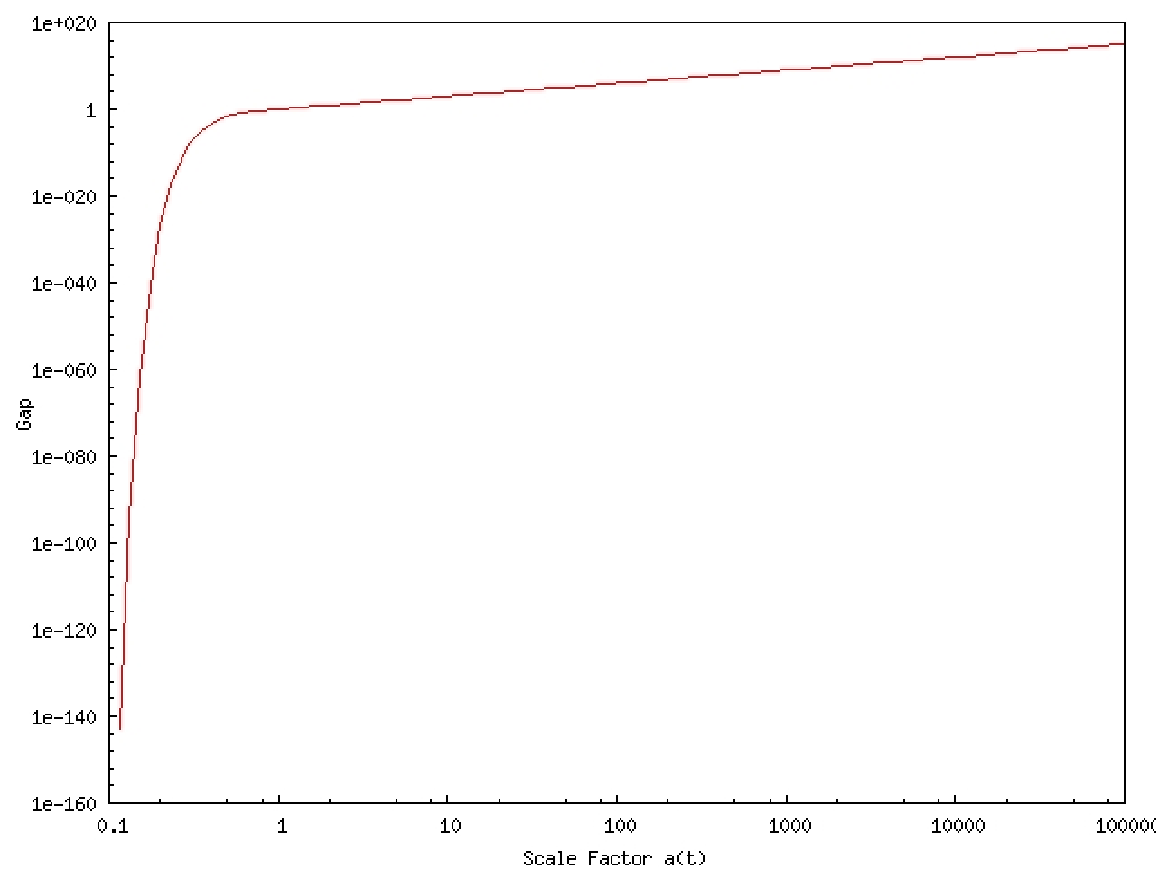
\includegraphics[keepaspectratio=true,scale=.4]{delta_plot.pdf}
%\caption{Condensate gap as a function of the scale factor} \label{fig:gap}
%\end{figure}

The gap has different behavior in the strong ($L \ll 1$) and weak ($L \gg 1$)coupling limits:

\begin{eqnarray}
    \Delta \sim \begin{array}{cc} \frac{2 \hbar
    \omega_D}{M^2_{pl}L^3}& L \ll 1\\2 \hbar
    \omega_D e^{-M^2_{pl}L^3}& L \gg 1\end{array}
%    \Delta \sim 2\hbar\omega_D \exp^{\frac{-1}{\alpha V_a D(0)}}  \quad \mbox{Weak coupling} \nonumber \\
 %   \Delta \sim 2\hbar\omega_D \alpha V_a D(0) \quad \mbox {Strong coupling} \nonumber \\
\end{eqnarray}

The gap is exponentially suppressed for large $L$ but is very large at early times when $L$ is very
small.

One has to keep in mind that this is a semiclassical calculation and breaks down for small $L$ as
we enter a non-perturbative regime where quantum gravitational fluctuations of the metric must be
taken into account.

\section{Discussion}

Eqn. (\ref{PotentialEnergy}) is the expression for the potential energy of the fermi gas. The gap
equation (\ref{GapEqn2}) has two solutions. The trivial solution is zero and corresponds to the
free fermi gas. In this case (\ref{PotentialEnergy}) reduces to the Hartree-Fock potential energy
for the free fermi gas \cite{Fetter2003Quantum}. When the condensate forms the potential is reduced by
the amount given by the last term in (\ref{GapEqn2})\footnote{The other terms in (\ref{GapEqn2})
are also affected when he have a condensate. However, this is perturbation is negligible compared
to the that due to the gap term}. The full Hamiltonian constraint (\ref{ReducedHamiltonian}) now
becomes:

\begin{eqnarray}\label{NewHamiltonian}
    \frac{1}{V}\int d^3x \,a^3 \,\mathcal{H} &=& -\frac{3}{\kappa}H^2 + \Lambda_0
        + \int \frac{d^3k}{(2\pi)^3} \left\{\sqrt{E_k^2 + \Delta_k^2}(m_k + \bar m_k + n_{-k} + \bar
        n{-k}) - \frac{2\Delta^2}{\sqrt{E_k^2 + \Delta_k^2}} \right\} \nonumber \\
        &=& -\frac{3}{\kappa}H^2 + \Lambda_0
        + \int \frac{d^3k}{(2\pi)^3} \sqrt{E_k^2 + \Delta_k^2}(m_k + \bar m_k + n_{-k} + \bar n{-k})
        - 2\frac{\Delta^2}{\alpha}
\end{eqnarray}

where $V$ is the volume of integration over the three-manifold. We have integrated the last term in
the first line using (\ref{GapEqn2}) and the assumptions listed below that equation.

Now we note that the second term in (\ref{NewHamiltonian}) corresponds to the quantized form of a
complex scalar field with mass $\Delta$. Hence we can replace that quantum expression with the
corresponding classical expression for a complex scalar field which the final form of the
Hamiltonian constraint:

\begin{equation}\label{FinalHamiltonian}
    \frac{3}{\kappa}H^2 = \frac{1}{2}\dot \Phi^2 + \Delta^2 \left(\frac{1}{2}\Phi^2 - \frac{2}{\alpha} \right)
\end{equation}

%The correction to the cosmological constant is given by two times the last term of
%(\ref{PotentialEnergy})\footnote{We have a contribution from the left and right handed spinors} :
%
%\begin{equation}\label{EffCC}
%    \Lambda_{corr} = 2\int \frac{d^3k}{(2\pi)^3} \frac{\Delta_k^2}{2 \sqrt{E_k^2 + \Delta_k^2}}
%    \approx \frac{2\Delta^2}{\alpha}
%\end{equation}

%where the third expression is obtained by using the approximation discussed at the end of the
%previous section.

where we have set $\Lambda_0$ to zero.

In \cite{Alexander2004} a perturbative one-loop calculation done for fermions coupled to gravity
via a quartic potential showed that the cosmological constant must be proportional to $\Delta^2$.
Here we have done a non-perturbative calculation to demonstrate that this expectation is indeed
borne out (if one ignores the bare cosmological constant).

%Also note that the last term in (\ref{NewHamiltonian}) is exactly the expression for the
%hamiltonian of two quantized complex scalar fields with a spatially varying mass\footnote{Once
%again we get two scalar fields because both $\xi$ and $\rho$ are non-zero}. This is due to the fact
%that the gap depends on the wave-vector. The approximation $\Delta_k = \Delta, \forall\,k$ yields a
%scalar field with a spatially constant (but time-dependent) mass. This approximation is made in
%order to facilitate the calculation of the gap. There is no other reason to set $\Delta_k$ to a
%constant. If, therefore, we retain the full expression (\ref{GapEqn2}) for $\Delta_k$ then what the
%above calculations yield is not only a negation of the bare cosmological constant but also two
%scalar fields with a spatially dependant masses. It is then tempting to speculate that the fourier
%modes of the mass term given by $\Delta_k^2$ are the much sought after perturbations that form the
%initial seeds of structure formation.

\section{Conclusion}

In this work we have demonstrated that when a covariant coupling to fermions in General relativity
induces a four fermion coupling, the Hamiltonian reduces to a BCS theory.  The gravitational field
also induces a chemical potential which creates a Fermi-surface.  By employing the appropriate
Boguliobov transformation we were able to diagonalize this Hamiltonian and evaluate the energy gap.
This gap plays the role of the mass of the scalar field corresponding to the condensate. In a time
dependent background the gap is time dependent. Hence if starts off in a very small volume, the
scalar field potential will source inflation. As the universe expands, the gap will decay until it
becomes negligible at which point inflation self-consistently ends. This scenario is explored in
more detail and supported by numerical calculation in \cite{Alexander2007Fine}.

There are questions this work raises that need to be explored further:
\begin{itemize}
    \item The fermions in our picture populate the universe before inflation, so they clearly
    cannot be Standard Model particles. What can be the origins of these fermions?
%All fermionic species, regardless of whether they couple to Yang-Mills or electromagnetic fields,
%also couple to gravity. Therefore a four-fermi interaction is induced for all fermions and does not
%distinguish between different species. In the real world we have fermions that condense (quarks)
%and those that are free (electrons and neutrinos). It remains to be understood how in this
%mechanism can one include interactions which would distinguish between different species, allowing
%some to condense and others to remain free.
%    \item How would the generic inflationary scenario be modified due to the presence of the gap?
%$<\bar\Psi\Psi>$ develops a non-zero vev and is a scalar. Can this composite scalar then play the
%role of the scalar field in cosmology?
    \item We assumed homogeneity and isotropy for our calculation. Gravitational perturbations
    would have an effect on the condensate. In particular if
$\Gamma^i_a$ (the spatial part of the connection) is non-zero then the number operator
(\ref{xiNumberOp}) would be modified by a term proportional to $e^a_i \Gamma_a^i$. This would
increase the chemical potential thereby decreasing $\Delta$. Thus inhomogeneities and anisotropies
would generically deplete the gap. Can one therefore argue that the homogeneity and isotropy of our
universe is a consequence of the fact that in an inhomogenous and anisotropic background,
inflation, with all its attending consequences such as leptogenesis structure formation which are
necessary for our universe to be the way it is, would not occur?
    \item The four-fermion interaction we use is not put in by hand but is an exact result of the
    equations of motion. However from an effective field theory point of view one can argue that in general
    higher dimension operators should also be allowed. We believe that such operators would not
    qualitatively change our conclusions. However a full effective action analysis needs to be
    performed in order to confirm this suspicion.
\end{itemize}

\section{Other Approaches}

\subsection{Covariant Approach} % contrast with Alexander-Biswas

\subsection{RG Approach}  % contrast with Neubert et al (a new model for the early universe)

\end{doublespace}

\chapter{Relaxation of Cosmological Constant}

\begin{doublespace}

\section{Introduction}

There are many faces to the cosmological constant/dark energy
problem.  First, the naive perturbative theoretical evaluation of
the vacuum energy of all particles in the standard model gives a
result that disagrees with observations by 120 orders of magnitude
\cite{Carroll2001Cosmological}. Second, a confluence of cosmological and
astrophysical observations, such as the WMAP satellite
\cite{Spergel2006Wilkinson} and Type Ia supernovae \cite{Astier2006Supernova},
indicate that the cosmological constant or something very similar to
it, currently dominates the universe.

Perhaps the most striking aspect of the cosmological constant
problem is seen in the details of the inflationary
paradigm \cite{Brandenberger2001Principles}. Inflation is driven by a
constant part of the Energy-Momentum tensor of a scalar field, which
is indistinguishable from a pure cosmological constant.  Therefore,
any mechanism which relaxes the cosmological constant would also
prevent inflation from happening. One way out of this possible
conundrum is to do away with fundamental scalar fields, allow
inflation to occur with a large cosmological constant and
investigate any self consistent mechanism which negates the
cosmological constant to almost zero.  Such a mechanism would solve
all three cosmological constant problems:


\begin{itemize}

\item The Cosmological constant would be dynamically relaxed due to the non-trivial dynamics of
inflation itself; it would be self regulatory.

\item Dark energy and the coincidence problem would be explained if a residual amount of
cosmological constant would be left over by the end of inflation.

\item Since inflation is not driven by a fundamental scalar fields, fine tuning of the cosmological
constant is no longer needed.

\end{itemize}

Attempts at tackling the this problem via cosmological condensates
include \cite{Brandenberger1997Asymptotic, Brout2003Condensation, Arkani-Hamed2004Ghost,
Alexander2004, Alexander2005A-Quantum}. More recently, Prokopec proposed a
mechanism involving a Yukawa coupling between a scalar field and
fermions \cite{Prokopec2006Solution}.

A simple way to obtain inflation in the absence of matter is due to
the presence of a non-zero, positive cosmological term on the right
hand side of Einstein's equation:

\begin{align}
    G_{ab} = 8\pi G \Lambda_0 g_{ab}\nonumber \\
   \Rightarrow a(t) = a_0 (t) e^{\sqrt{\frac{\Lambda_0}{3}}t}
\end{align}

where we have used the FRW metric ansatz to obtain our solution.
$a(t)$ is the scale factor.  From the solution it is clear that the
Hubble rate $H = \sqrt{\frac{\Lambda_0}{3}}$.

While this simple model gives us an inflating universe it is clearly
not in line with reality because it does not predict an end to
inflation.  A way to get around this obstacle is to introduce
matter, traditionally scalar fields, into the picture. Then the
first Friedmann equation becomes:

\begin{equation}
    3\left( \frac{\dot a}{a} \right)^2 = \Lambda_0 + \frac{1}{2}
    \dot \phi^2 + V(\phi)
\end{equation}

where $\phi$ is the scalar field.

We also have the E.O.M for the scalar field:

\begin{equation}
    \ddot \phi + 3 \frac{\dot a}{a} \dot \phi + \frac{dV}{d\phi} = 0
\end{equation}

where $V(\phi)$ is the scalar field potential. Such models typically
require special initial conditions for the scalar field called the
"slow-roll" conditions. The scalar field must start off at a large
initial value and then start rolling slowly down an almost flat
potential. This results in an inflationary universe. After a
sufficient number of e-foldings, the scalar fields reaches the
steeper part of the potential where it decays via parametric
resonance leading to reheating and particle production after
inflation has ended.

Unfortunately, such models have several shortcomings:
\begin{itemize}
  \item The shape of the potential is arbitrary and we have no physical way of choosing
  the one that would correspond to our universe from an almost
  infinitely large family.
  \item We require the scalar field to start off at a large initial
  value. What mechanism would cause the scalar field to be "pumped
  up" to this value initially?
  \item The mass of the scalar field is an arbitrary parameter. It
  can be fixed once we fix the potential, but it remains a source of
  vagueness.
  \item Most importantly, from whence did this scalar field come
  . Perhaps if one tries to tackle this fundamental question head
  on the others might also be amenable to a solution.
\end{itemize}

In this letter we propose a dynamical solution to the CC problem
assuming only the Standard Model and General Relativity.  There are
no fundamental scalar fields to tune.  Therefore the universe will
be dominated by a large cosmological constant, which naturally
generates inflation.  The non-trivial observation here is that the
dynamics of inflation itself holds the key to relaxing the
cosmological constant without fine tuning. How is this possible? The
exponential time dependent behavior of de Sitter space
counterintuitively enhances correlations between fermion pairs.
These correlations become so strong that these fermions form a
Cooper pair.

In a recent paper \cite{Alexander2006Gravity}, we showed how the presence
of torsion and fermionic matter in gravity naturally leads to the
formation of a fermionic condensate with a gap which depends on the
3-volume.  In this letter we will analyze explicitly the dynamics of
the universe with a cosmological constant in the presence of this
gap. Numerical calculations then show that with a large initial
cosmological term and generic initial conditions for the scalar
field and its momenta, we obtain a universe which undergoes an
inflationary phase during which the gap grows as a function of
$a^3$, causing the effective cosmological term to diminish to a
small positive value.

In Section 2 we discuss the E.O.M for our system. In Section 3 we
present the numerical results and finally we conclude with some
discussion or our results and what they imply for our understanding
of inflation and the cosmological term.

\section{Friedmann and scalar equations}

We briefly summarize the steps that were taken in
\cite{Alexander2006Gravity}. We started with the Holst action for gravity
with fermions:

\begin{equation}
    S_{H+D} = \frac{1}{2\kappa}\int d^{4}x\,e(\,e^{\mu}_{I}e^{\nu}_{J}R^{IJ}_{\mu\nu} - \frac{2}{3}\Lambda_0) -
    \frac{1}{2\kappa\gamma}\int d^{4}x\,e\,e^{\mu}_{I}e^{\nu}_{J}\star R^{IJ}_{\mu\nu} + \frac{i}{2}\int d^{4}x\,e\,(\bar{\Psi}\gamma^{I}e^{\mu}_{I}D_{\mu}\Psi -
    \overline{D_{\mu}\Psi}\gamma^{I}e^{\mu}_{I}\Psi)
\end{equation}

$e^\mu_I$ is the tetrad field. $R_{\mu\nu}^{IJ}$ is the curvature
tensor. The second term in the above equation is analogous to the
$\Theta$ term in Yang-Mills theory and is required if we want to
work with arbitrary values of the Immirzi parameter ($\gamma$).
After varying the action w.r.t the connection $A^\mu_{IJ}$ and
solving the Gauss constraint we which that $A^\mu_{IJ} =
\omega^\mu_{IJ} + C^\mu_{IJ}$\footnote{Which implies that the
torsion is non-zero}, where $\omega^\mu_{IJ}$ is the tetrad
compatible connection and $C^\mu_{IJ}$ can be expressed in terms of
the axial vector current:

\begin{equation}
    C_\mu^{IJ} = \frac{\kappa}{4}\frac{\gamma^2}{\gamma^2 + 1}j^M_a\left \{ \epsilon_{MK}{}^{IJ}e^K_\mu
            - \frac{1}{2\gamma}\delta^{[J}_M e^{I]}_\mu \right\}
\end{equation}

where $ j^M_a = \bar\Psi\gamma_5\gamma^M\Psi$. Inserting the torsion
into the first order action we find the resulting second order
action which now contains a four-fermi interaction and the tetrad is
the only independent variable, the connection having already been
solved for in the previous step.

\begin{equation}
    S[e,\Psi] = S_{H+D}[\omega(e)] -\frac{3}{2}\pi G \frac{\gamma^{2}}{\gamma^{2}+1} \int d^{4}x\,e (j_a^I)^2
\end{equation}

Then we did the 3+1 decomposition of the action to find the
Hamiltonian, which after making the ansatz of a FRW metric becomes:

\begin{eqnarray}
\label{ham}
    {\cal H} &=& -\frac{3}{\kappa}a^3H^2 +
    a^3\Lambda_0 + \frac{i}{a}\big(\psi_L^\dag\sigma^a\partial_a\psi_L - \psi_R^\dag\sigma^a\partial_a\psi_R\big) \nonumber \\
    &+& \frac{3\kappa}{32a^3}\frac{\gamma^2}{\gamma^2+1}\left[\psi_L^\dag\psi_L - \psi_R^\dag\psi_R\right]^2 = 0
\end{eqnarray}

We see that the right hand side is the sum of the gravitational,
Dirac and interaction terms. $\psi_L (\psi_R)$ is the spinor for
left (right) handed fermions. $\gamma$ is the Immirzi parameter. $H
= \frac{\dot a}{a}$ is the Hubble rate.

The key ingredient that dynamically cancels the cosmological
constant arises from the four-fermion interaction in the r.h.s of
(\ref{ham}).  This effect arises from an interplay between general
covariance and non-perturbative quantum mechanics.  General
covariance guarantees the four-fermion interaction.  What about the
non-perturbative quantum mechanics?  We see that the effective
coupling of the four-fermion interaction becomes large for small
values of the scale factor (ie. at early times).  The form of this
Hamiltonian maps directly into the BCS Hamiltonian of
superconductivity, except it is the gravitational field that is
playing the role of the phonons. As a result, just like in the BCS
theory (see eg. \cite{Fetter2003Quantum}), an energy gap $\Delta$ opens
up which reflects the instability of the ground state associated
with the bare cosmological constant.  An effective cosmological
constant with a lower energy is generated from the formation of the
gap.  To obtain the gap, we diagonalize the fermionic part of this
Hamiltonian by expanding the fermions in normal modes and using a
Boguliubov transformation. The resulting Hamiltonian is:

\begin{eqnarray}
\mathcal{H} &=& -\frac{3}{\kappa}H^2 + \frac{1}{\kappa}(\Lambda_0 -
\Lambda_{corr})
        + \nonumber \\
         && \int \frac{d^3k}{(2\pi)^3} \sqrt{E_k^2 + \Delta^2}(m_k + \bar m_k + n_{-k} + \bar
        n_{-k})
\end{eqnarray}

where the non-perturbative correction to the bare cosmological
constant is\footnote{$\Delta$ is obtained by solving the gap
equation obtained in \cite{Alexander2006Gravity} in a self-consistent
manner}:

\begin{eqnarray}\label{gap1}
    \Lambda_{corr} & = & 2 \Delta^2 \nonumber \\
    \Delta & = & \frac{2\hbar\omega_D \exp^{\frac{\nu}{2}}}{\exp^{\nu} - 1}
    \qquad \left(\nu = \frac{2}{\kappa\, a^3 k_f^2}\frac{\gamma^2 + 1}{\gamma^2} \right)
\end{eqnarray}

$k_f$ is the fermi energy, $E_k$ is the energy of the $k^{th}$ mode
of the condensate and $\gamma$ is the Immirzi parameter. $m_k (n_k)$
and $\bar m_k (\bar n_k)$ are the creation (annihilation) operators
for the condensate of the left and right-handed fermions
respectively. The $a^3$ factor in $\Delta$ comes from the fact that
the density of states in an expanding universe scales as the
3-volume. We see that the last term in the Hamiltonian constraint
corresponds to the quantized expression for a scalar field
condensate, $\phi_{c}$, with mass $\Delta$ \footnote{To be precise
we note that there are \emph{two} scalar fields, corresponding to
the two pairs of annihilation and creation operators. However in the
following we use only one scalar field for simplicity. Noting that
the left handed massless fermions are the antiparticles of the right
handed ones, we can conjecture that this expression is the quantized
form of a \emph{complex} scalar field, which would imply that we are
dealing with an axion}. Replacing this with the classical expression
for a scalar field we get:

\begin{equation}
    \mathcal{H} = -\frac{3}{\kappa}H^2 + \frac{1}{\kappa}(\Lambda_0 - \Lambda_{corr})
        + \frac{1}{2}\dot\phi_c^2 + \frac{1}{2}\Delta^2 \phi_c^2 = 0
\end{equation}

It is important to keep in mind that $\phi_c$ is not a fundamental
scalar field. Its annihilation and creation operators ($m_k$ and
$n_k$) correspond to excitations of the condensate. This leads to
the first Friedmann equation with a time-dependent correction to the
cosmological constant and a scalar field as our matter:

\begin{equation}\label{friedmann_eom}
    3\left(\frac{\dot a}{a}\right)^2 = \Lambda_0 - \Lambda_{corr}
        + \frac{1}{2}\dot\phi_c^2 + \frac{1}{2}\Delta^2 \phi_c^2
\end{equation}

after setting $\kappa = 1$.

The equation of motion for a scalar in a FRW background is:

\begin{equation}\label{scalar_eom}
    \ddot \phi_c + 3\frac{\dot a}{a}\dot \phi_c + \Delta \phi_c^2 = 0
\end{equation}

We see that the energy gap (\ref{gap1}) increases monotonically with
$a$. From this we can guess the qualitative behavior of the scale
factor.  As long as the initial value of the scale factor is such
that $2 \Delta^2 < \Lambda_0$, then from (\ref{friedmann_eom}) we
see that the right hand side will be positive definite resulting in
an inflating universe. The Hubble rate plays the role of friction
for the scalar field. As time develops the friction will drive $\dot
\phi_c$ to reach zero.  From then until inflation ends, $\phi_c$
will be a constant. Eventually the scale factor becomes large enough
and the right side of (\ref{friedmann_eom}) will start to decrease.
$H$ will then decrease and reach its minimum when:

\begin{equation}\label{critical_gap}
 \Lambda_0 = 2 \Delta^2  -  \frac{1}{2}\Delta^{2}\phi_{c}^{2} -
 \frac{1}{2}\dot \phi_c^2
\end{equation}

$\phi_c$ will then start rolling down the potential hill again,
which is becoming steeper because $a(t)$ and hence $\Delta$ is still
increasing. This presence of the scalar condensate coupling in the
r.h.s of (\ref{critical_gap}) means that when the system dynamically
relaxes to $\Lambda_{eff} = 0$,   it is in a state in which the
energy density of the effective cosmological constant
$\Lambda_{eff}=\Lambda_{0}-2 \Delta^2 $ traces the energy density of
matter.   This condition is similar to the relaxation mechanism due
to backreaction of IR gravitational waves in which the backreaction
effects ceases to negate the cosmological constant and one reaches a
scaling solution where the energy density of matter and radiation
traces the effective cosmological constant\cite{Brandenberger2002BackReaction,
Abramo1999Cosmological}. We will see in the next section that once the
cosmological constant is canceled the tracking solution is
dynamically reached without any fine tuning and the cosmological
constant will remain vanishingly small.

We can see that the kinetic energy of the scalar field will
dissipate eventually, due to a small but non-zero $H$. $H = 0$ is
the late-time attractor for this system. As $a(t)$ increases, the
R.H.S. of (\ref{friedmann_eom})will decrease and eventually reach
zero. The solution is stable with respect to perturbations around
this point because of the presence of the gap.

The expression (\ref{critical_gap}) allows us to calculate the value
of the scale factor at the end of inflation. For large $a$, $\Delta
\sim a^3 M_{pl}^2 k_f^2 $. Then from (\ref{critical_gap}) we have:

\begin{equation}\label{final_a}
    a_f = \left ( \frac{\Lambda_0 M_{pl}^2}{2 E_D^2 k_f^4} \right)^\frac{1}{6}
\end{equation}

where $E_D = \hbar \omega_D$. Then for the number of e-foldings we
find:

\begin{equation}\label{efoldings}
    N = ln\left( \frac{a_f}{a_i} \right) \sim - \frac{1}{6} ln(E_D^2 k_f^4)
\end{equation}

where we have set the scale factor at the beginning of inflation
$a_i = 1$. If we assume that $E_D \sim M_{pl}$ and $N = 60$ then
this implies that $k_f \sim e^{-90}$.


\section{Numerical solution and results}

For our numerical calculation we work in Planck units ($\kappa \sim
M_{pl}^2 = 1$). We set $E_D$ and $k_f$ to be $M_{pl} \sim 1$. We
must emphasize that the qualitative behavior is completely
independent of the values of these parameters. In particular, if we
set $k_f = e^{-90}$ we would get 60 e-foldings. It is reasonable to
assume that the bare cosmological constant cannot exceed $M_{pl}^4$
and thus we set $\Lambda_0 = M_{pl}^4 \sim 1$. Then the expression
for the gap becomes:

\begin{equation}\label{gap}
    \Delta = 2\frac{\exp^{\frac{1}{a(t)^3}}}{\exp^{\frac{2}{a(t)^3}} - 1}
\end{equation}

\begin{figure}[htp]\label{fig:gap} 
\centering
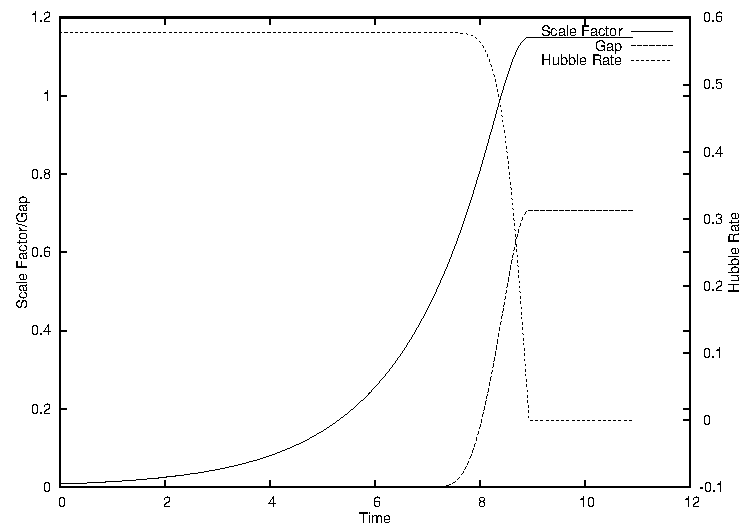
\includegraphics[scale=0.6]{figures/cosmological_condensate/simplot.pdf}
\caption{Scale factor, hubble rate and condensate gap as a function of time}
\end{figure}

We solved equations (\ref{scalar_eom}) and (\ref{friedmann_eom})
numerically. An analytic solution is not possible because of
non-analytic form of the gap (\ref{gap}). Fig. \ref{fig:gap} shows
the behavior of the scale factor and the hubble rate as a function
of time.

We find that initially the universe undergoes inflationary expansion
(indicated by the constant value of the hubble rate). When the gap
becomes large enough to cancel out the bare cosmological constant,
inflation ceases.

The behavior of the scalar field and momentum is in accord with the
expectations outlined in the previous section. The scalar field
increases or decreases initially depending on the sign of the
initial value of the scalar momentum. It quickly levels off to a
constant value for the rest of the inflationary period, as the
momentum is driven towards zero by a positive $H$ and stays there
until inflation ends. This behavior is independent of the initial
values (which ranged from $0.5$ to $-0.5$ in various runs) and shows
that during inflation the Hubble rate during inflation is always
$\sqrt{\Lambda_0}/3$. In fact, the scalar field plays no role in the
relaxation of the bare cosmological constant. A numerical
calculation setting $\phi_c = \dot \phi_c = 0$ confirms this. Fig.
\ref{fig:scalar} shows the scalar field evolution for one set of
initial values.

\begin{figure}[htp]\label{fig:scalar_field}
\centering
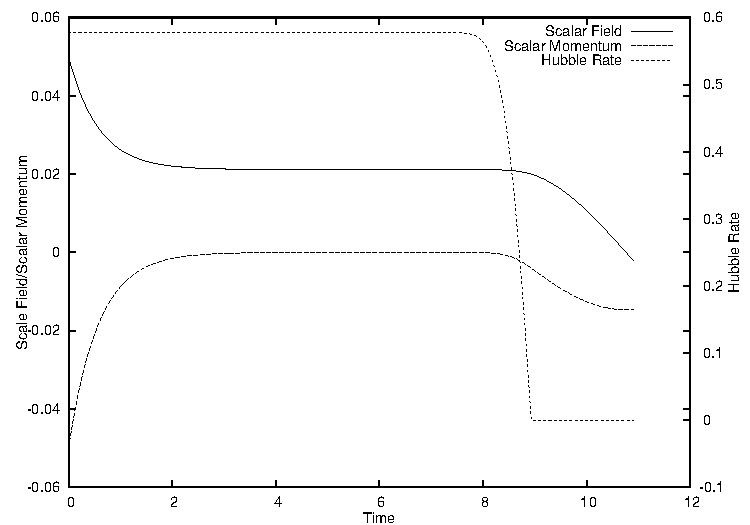
\includegraphics[scale=0.6]{figures/cosmological_condensate/scalar.pdf}
\caption{Scalar field and momentum}
\end{figure}


\section{Discussion}

In a universe filled with fermions and with a positive cosmological
constants is unstable. Their exists an interaction between fermions
propagated by torsion at the level of the effective field theory.
This interaction leads to the formation of Cooper pairs and a
condensate forms whose free energy is lower than that of the
deSitter background. Consequently the bare cosmological constant,
which we identify to be the free energy of the deSitter background,
is lowered by an amount proportional to the square of the condensate
gap. We have cosmic expansion because initially the gap does not
cancel out the bare cosmological constant completely. The size of
the gap depends on the 3-volume. Hence as the expansion occurs the
effective cosmological "constant" becomes smaller, until eventually
after a period of inflation we emerge from the deSitter vacuum into
flat Minkowski space, where $H \sim 0$.

The number of e-foldings during inflation is given by
(\ref{efoldings}) and can be tuned by adjusting $E_D$ and $k_f$. The
behavior of the scale factor is also independent of the scalar field
evolution.

There are three free parameters in our model. The bare cosmological
constant $\Lambda_0$, the fermi energy $k_f$ and the Debye energy
$E_D$. In a condensate $E_D$ is the cutoff frequency and is
determined by the lattice size. In a cosmological context therefore
we can speculate that it should be $\sim M_{pl}$. $k_f$ can
constrained according to (\ref{efoldings}) to be $\sim e^{-90}$.
$\Lambda_0$ determines the Hubble rate during inflation. From the
WMAP data \cite{Spergel2006Wilkinson}, the upper limit on $H/M_{pl}^2$ is
constrained to be $10^{-4}$. From this we can deduce that the bare
cosmological constant, needs to be fixed by hand to be $\Lambda \sim
H^2 \sim 10^{-8} M_{pl}^4$ in order to conform to observations.

We have presented here a non-perturbative mechanism which relaxes
the bare cosmological constant to zero.  As a bonus we find that the
relaxation is accompanied by an inflationary period. The duration of
inflation is determined by two parameters ($E_D$ and $k_f$) whose
precise determination requires physics beyond the standard model.
The lack of fine-tuning is demonstrated by the fact that the
solution has an attractor with $H=0$ independent of the values of
the free parameters.

The scalar field discussed here is an emergent degree of freedom.
After inflation, oscillations of this field can lead to reheating.
However, to what extent this would be a viable description of the
post-inflationary period remains to be seen in future work.

\end{doublespace}

\chapter{Alternatives to Dark Energy}

%\begin{doublespace}

\section{Introduction}

It is important for researchers in dark energy, and cosmology in general, to be familiar with the observational basis for claims regarding the most appropriate cosmological model. Perhaps the weakest link in the chain of observation and reasoning leading to the LCDM model, lies in the assumptions used to determine luminosity distances between Earth and the various astronomical objects that serve as ``standard candles". These calculations are commonly done with the assumption of large-scale homogeneity in the visible universe. Recent evidence (\cite{York2000The-Sloan,Abazajian2009The-Seventh,Percival2001The-2dF-Galaxy}) highlighting the complexity in the large-scale structure (\cite{vandeWeygaert2009Geometry,vandeWeygaert2004Hierarchy,Shandarin2004Morphology}), conclusively demonstrates that we live in a universe whose evolution during the current epoch cannot be described by linear perturbation theory. Such an approach is applicable from the time of the last scattering surface ($ t_{rec}$) upto the earliest stages of star and galaxy formation ($ t_{struct} $). Past that stage, regions with a large enough density contrast have formed whose further evolution requires non-linear methods along the lines of those used to describe dark matter halo evolution (\cite{Giocoli2007An-improved}) . Once regions with large enough density contrast\footnote{$ |1-\rho/\overline{\rho}| \gtrsim 0.1 $; the ratio between the local matter density and the large-scale averaged density} have formed the next phase in the evolution involves processes of collisions between these regions, leading to the formation of galaxy clusters connected by filaments of matter, a structure collectively referred to today as the ``Cosmic Web".

This magnificent structure can be thought as the scaffolding of our universe. It resembles a foam-like fluid containing voids (regions of under-density) between which are sandwiched sheets of matter forming one-dimensional filamentary structures which join up at cosmic ``nodes" which can be identified as regions with active star formation.

One reason for the success of the LCDM model is that the propagation of light through these complex structures appears to be an analytically intractable problem. Various arguments have been made in the literature [\textbf{find and cite refs}] justifying the assumption of homogeneity, even though regions with a density contrast as high as $ \pm 0.3 $ are known to exist in our cosmic neighborhood. For the greater portion of the time it takes a photon to travel from $ t_{rec} $ to the present epoch, it travels through a universe which is far from homogenous. The strongest assumptions of homogeneity can be imposed only when comparing structures at the same scale, and even then the weaker criterion of self-similarity rather than homogeneity is more applicable.

Once we pick a scale $ k_{rec} $ for density perturbations at $ t_{rec}  $, it can be argued that whatever structures that have formed at the present time at the scale $ k_{now} $ ( corresponding to a redshifted $ k_{rec} $ ) are likely to be similar in shape and composition. For instance, if we pick a scale of 1 cm [\textbf{check ???}] at $ t_{rec} $, which corresponds to a present day scale of $ \sim $ 30 Mpc [\textbf{check}], then we can safely say that were we to sample the library of structures in the present day universe for structures at that \emph{fixed} scale, we would find morphological and compositional similarities between them. This in no way implies that were we to compare structures at different scales \emph{during the same epoch}, say $ \sim $ 300 Mpcs and $ \sim $ 30 Mpc, would we would find any similarity or homogeneity.

It is only in this restricted sense that one can argue for homogeneity! The moment we consider comparing structure at different scales we are bound to run into trouble, because \emph{the cosmos is not scale-invariant}. When considering the propogation of a photon from the time of recombination until today it is clear that its path passes through many different scales at different epochs, whose structure and composition becomes more delineated as we reach closer to the present epoch. Therefore, in the absence of an investigation into the effects of inhomogeneities on luminosity distances, the LCDM model remains standing as the best model we \emph{have} as opposed to the best model which \emph{can be} determined by the complete range of cosmological observations.

It is fortunate, that such investigations have been initiated by a number of individuals are groups. Notable among are Celerier \cite{Celerier2007Do}, Inoue and Silk \cite{Inoue2006Local,Inoue2007Local}, Biswas, Mansouri, and Notari \cite{Biswas2006Nonlinear} among others. In most cases, in lieu of an analytical handle on inhomogeneities along the \emph{entire} history of the photon, one generally considers an approximation where the local patch of the cosmos, which includes our Milky Way, is a region of under-density. Our ``local void" is surrounded by sheets of matter on its boundary parts of which could conceivably be identified with the structure known as the ``Great Wall" in the SDSS. Such a geometry, consisting of a void bounded by a shell of matter embedded in a larger FRW background, can be analytically described by what is known as an Lemaitre-Tolman-Bondi (LTB) metric after the names of its originators, embedded in a large FRW universe. This is the the first step in the direction of a complete non-perturbative treatment.

In the following sections we describe in turn, an overview of the theory of hierarchical structure formation, the calculation of luminosity distances for photons in inhomogeneous space-times, the geometry of the LTB metric and the constraints that present day CMB data places on the size and shape of our local void.

\section{Cosmic Candles and Luminosity Distance}


\section{Parameter Estimation using Markov Chain Monte Carlo (MCMC)}

Large sample space
Statistical method of finding a solution
Bayesian analysis => Estimating parameters given a theory and a data set
Markov Chain => Particular method used
Software => CosmoMC by Sarah Bridle and Antony Lewis
Dataset => WMAP ver. 3
Hardware => On PSU HPC cluster (lionxl)

\section{Comparison with LCDM model}

Likelihood tables

\appendix

\section{Microwave Background Radiation from Cosmic Anistropies}

\textbf{summarize derivation of CMB via boltzmann's equation from chap. 9 of mukhanov}

\begin{figure}[htbp]
\begin{center}
		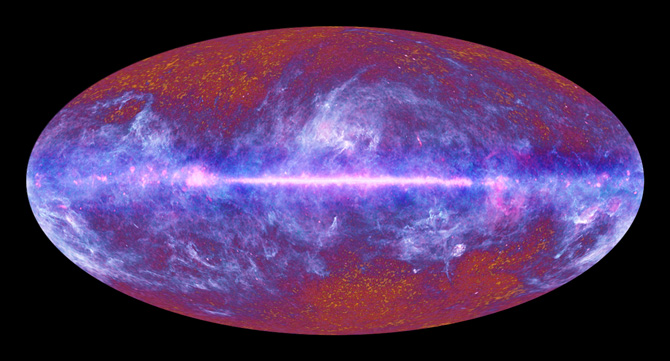
\includegraphics[scale=0.3]{figures/voids/planck_fullsky}
		\caption{A full sky map of the Cosmic Microwave Background as seen by the \textit{Planck} satellite [2010]}
		\label{fig:planck_fullsky}
\end{center}
\end{figure}

\section{LTB Model}

\section{Hierarchical Structure Formulation}

Structure formation is a highly non-linear process. It cannot be understand by the simple linear theory of wavelengths entering the horizon at different redshifts. However, numerical simulations are not the viable only line of attack. There exists an analytical framework centered around Smulochowski's work on fluctuations. The essential idea is that when we look at the ``entire universe", the matter density distribution shows no fluctuations. However, as we look at smaller and smaller scales, the fluctuations in the matter density $ \frac{\delta \rho }{\rho} $ increase and become more random. This variation of the density with scale can be viewed as a brownian walk - and this is where Smoluchowski's work comes into play.

%Now the critical density of a distribution of matter above which gravitational collapse overwhelms the background cosmological expansion varies with scale (... exactly why ?). 

The fluctuation spectrum is embedded in the initial conditions - at recombination - and depends on the inflationary model used. But essentially it can be fixed by hand, not worrying about what form of inflation created it. This initial condition then determines the future evolution of the matter density and halo formation. Even though the resulting evolution is statistical, it is not indeterminate. The distribution of halos at different redshifts depends on the fluctuation spectrum specified as part of the initial conditions.

The insights from the work on halo formation, from Press-Scheter to Sheth and Moreno, can be summarized as follows:

1. The halo size distribution as a function of redshift is a member of a statistical ensemble that is characterized by the initial conditions.

%2. Halo formation and growth is a highly non-linear process, which can be modeled accurately using Smulochowski's work on fluctuation theory.

3. Given a halo of a certain size at a certain redshift, one can trace its history backwards in time. As we decrease z, the halo shrinks, eventually reaching a point where its size is smaller than the critical density at that red-shift, and it then splits (most commonly into two pieces). Each branch can then be recursively processed to yield a fractal model of halo formation.

4. Halo formation exhibits scaling relations and universality. We can consider halos of mass m and m' and evaluate the corresponding critical densities of formation as a function of redshift. With an appropriate scaling we find that the two curves coincide.

Halo formation is a non-linear process, exhibiting self-similarity and universality!

The net effect of these considerations can be best summarized by Fig. \ref{fig:MilleniumSimulation} taken from \cite{Springel2006The-large-scale,Springel2005Simulating}.

\begin{figure}[hbtp]
	\centering
	\subfigure{
	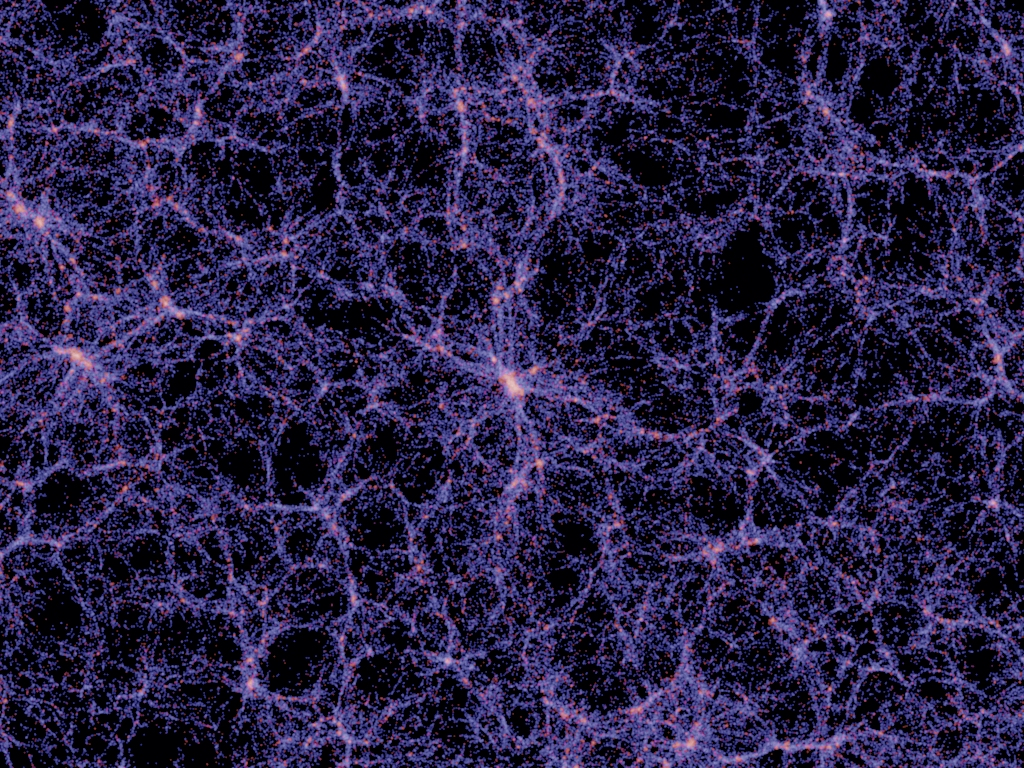
\includegraphics[scale=0.15]{figures/voids/galseq_D_063}
%	\label{fig:GalDistSim}
}
	\subfigure{
	\includegraphics[scale=0.15]{figures/voids/seqD_063a_half}
%	\label{fig:DarkMatterDistSim}
}
	\caption{The large scale distribution of visible matter (left) and dark matter (right) in the present epoch as modelled by the Millenium Simulation}
	\label{fig:MilleniumSimulation}
\end{figure}

\section{Cosmological Averaging}

Summarize Buchert and Wiltshire's work.

\section{Discussion}

There has been no lack of criticism of this model of apparent cosmic acceleration, much of which centers around the notion that our location near the center of a large void is in conflict with the cosmological principle and with precision cosmological measurements. For instance the abstract of one such rebuttal \cite{Moss2010Precision} begins with the statement that

"The suggestion that we occupy a privileged position near the centre of a large, nonlinear, and nearly spherical void has recently attracted much attention as an alternative to dark energy. ...."

In this and similar rebuttals the issue of our ``privileged position" near the center of a void is often raised as a philosophical objection to the model. However, contrary to common opinion, our location in the interior region of a void is not only likely but also necessary from an anthropic point of view. In fact, one can go on to argue that life-bearing systems are far more likely to occur in the relatively quiet interiors of voids rather than in the filaments or nodes of the cosmic web which are regions of star formation and hence full of highly energetic debris which would make the uninterrupted evolution of life on a planet over many eons unlikely.

Such an argument is amenable to experimental confirmation or rejection by looking at the results of the various exoplanetary searches in progress. In addition the results of void-finder models \cite{Colberg2008The-Aspen-Amsterdam} consistently show that \emph{the basic results of the various methods agree very well with each other in that they all locate a major void near the centre of our volume}.

Ultimately whether or not the void model rules out the existence of dark energy is not by itself the major issue at stake here. It is irrefutable that the inhomogeneous large-scale structure of the galactic web must figure into any complete analysis of CMB or other cosmological data.

%\end{doublespace}

\chapter{Conclusion}


%% now we include the appendices
\appendices
%% omit this if there are no appendices

%% if there is only one appendix, 
%% say \singleappendix instead of \appendices
% \singleappendix

%% these are the actual commands to include the apendix files:

\include{app-bcs-gravity}

%\include{app-voids}

%\include{ap-more}


%% finally comes the bibliography and vita
%% the bibliography is generated automatically using BibTeX
%% Note: in order to get the (author year) citation style, this example 
%% includes a different *.bst style file than psuthesis.bst.  Sarah found 
%% this style file on: http://www.ee.oulu.fi/~harza/latex/  
%% This style includes the paper titles in the bibliography, so use it 
%% if you want:
%\bibliographystyle{/enter/path/to/ayphdthesis_mod}
%% However, according to the grad school thesis guide (c.2004), there is no 
%% special formating required for the bibliography, and to just follow 
%% the citation styles of your field, in that case the ``apj'' style is 
  %% prefectly OK, so that is the one that is going to be included in this
%% example file (use whichever style you prefer):
\bibliographystyle{jhep3}

%% the following is the path to you *.bib file 
%% (you do not need to enter the ``.bib'' extention)
\bibliography{../bib_library}
%% ADS can generate the entries in the bib file for you, just call up
%% the abstract, then near the bottom of the abstract page there is a
%% link to ``Bibtex entry for this abstract'' - just copy that into 
%% your bib file.  Here is an example bibtex entry:
%% @ARTICLE{citecode,
%%    author = {{Smith}, J. and {Jones}, M.},
%%     title = "{This Paper has some Really Cool Results}",
%%   journal = {\aj},
%%      year = 2002,
%%     month = sep,
%%    volume = 123,
%%     pages = {1-20},
%%    adsurl = {http://adsabs.harvard.edu/cgi-bin/nph-bib_query?bibcode=2002AJ....123.1S&amp;db_key=AST},
%%   adsnote = {Provided by the NASA Astrophysics Data System}
%% }
%% NOTE: ADS returns the AASTeX code for the journal name, you'll either 
%% have to change that by hand in each bib entry, or include a 
%% definition of the codes in your ``definitions'' file so LaTeX doesn't 
%% freak out.  Also, what I entered as ``citecode'' can be changed to 
%% whatever you want to use in the citations in the document, i.e., for
%% ``\citet{citecode}'' or ``\citep{citecode}''.


%% the thesis must end with a Curriculum Vitae (**one page or less**)
%% (this is Sarah's formatting, not sure how it compares to the other examples)
% LaTeX Curriculum Vitae Template
%
% Copyright (C) 2004-2009 Jason Blevins <jrblevin@sdf.lonestar.org>
% http://jblevins.org/projects/cv-template/
%
% You may use use this document as a template to create your own CV
% and you may redistribute the source code freely. No attribution is
% required in any resulting documents. I do ask that you please leave
% this notice and the above URL in the source code if you choose to
% redistribute this file.

\documentclass[letterpaper]{article}

\usepackage{hyperref}
\usepackage{geometry}

% Comment the following lines to use the default Computer Modern font
% instead of the Palatino font provided by the mathpazo package.
% Remove the 'osf' bit if you don't like the old style figures.
\usepackage[T1]{fontenc}
\usepackage[sc,osf]{mathpazo}

% Set your name here
\def\name{Deepak Vaid}

% Replace this with a link to your CV if you like, or set it empty
% (as in \def\footerlink{}) to remove the link in the footer:
\def\footerlink{}

% The following metadata will show up in the PDF properties
\hypersetup{
  colorlinks = true,
  urlcolor = blue,
  pdfauthor = {\name},
  pdfkeywords = {physics, gravity, cosmology, quantum field theory},
  pdftitle = {\name: Curriculum Vitae},
  pdfsubject = {Curriculum Vitae},
  pdfpagemode = UseNone
}

\geometry{
  body={6.5in, 8.5in},
  left=1.0in,
  top=1.25in
}

% Customize page headers
\pagestyle{myheadings}
\markright{\name}
\thispagestyle{empty}

% Custom section fonts
\usepackage{sectsty}
\sectionfont{\rmfamily\mdseries\Large}
\subsectionfont{\rmfamily\mdseries\itshape\large}

% Other possible font commands include:
% \ttfamily for teletype,
% \sffamily for sans serif,
% \bfseries for bold,
% \scshape for small caps,
% \normalsize, \large, \Large, \LARGE sizes.

% Don't indent paragraphs.
\setlength\parindent{0em}

% Make lists without bullets
\renewenvironment{itemize}{
  \begin{list}{}{
    \setlength{\leftmargin}{1.5em}
  }
}{
  \end{list}
}

\begin{document}

% Place name at left
{\huge \name}

% Alternatively, print name centered and bold:
%\centerline{\huge \bf \name}

\vspace{0.25in}

\begin{minipage}{0.45\linewidth}
  A-16, 1st Floor (East Facing) \\
  South Extension, Part II \\
  New Delhi - 110049 \\
  India
\end{minipage}
\begin{minipage}{0.45\linewidth}
  \begin{tabular}{ll}
    Phone: & +91-9717275953 (Cell) \\
     &  +91-11-65363116 (Landline)\\
    Email: & \href{mailto:dvaid79@gmail.com}{\tt dvaid79@gmail.com} \\
    Homepage: & \href{http://www.phys.psu.edu/people/display/index.html?person_id=1861}{\tt Link} \\
  \end{tabular}
\end{minipage}


\section*{Personal}

\begin{itemize}
\item Citizen of India
\end{itemize}


\section*{Education}

\begin{itemize}
  \item B.S. Physics, University of Missouri at Rolla\footnote{now known as Missouri University of Science and Technology }, 2000--2003
  \item Ph.D. Physics, Pennsylvania State University, 2003--2011, (defended Nov. 2010, completion Oct. 2011)
\end{itemize}


\section*{Research Experience}

\subsection*{Doctoral Research}
\begin{itemize}
\item \textbf{Independent study}, Advisor: Prof. Abhay Ashtekar, Topic: \emph{Geometric Quantum Mechanics}; Pennsylvania State University, (2004--2005)
\item \textbf{Independent study}, Advisor: Prof. Martin Bojowald; Pennsylvania State University, (2005--2006)
\item \textbf{Thesis research}, Advisor: Prof. Stephon H. S. Alexander, Pennsylvania State University, (2006--2010). Research topics covered include:
\begin{enumerate}
\item Studying the effects of LTB metric on anisotropies of the Cosmic Microwave Background using WMAP3 data
\item Applying Markov Chain Monte Carlo (MCMC) to obtain likelihood for Cosmological model fits to WMAP3 data.
\item Condensation of fermions in a cosmological setting
\item Generating Inflation from Condensates
\item Cosmological Parameter Extraction from WMAP3 data via Bayesian Analysis 
\end{enumerate}
\end{itemize}

\subsection*{Undergraduate Research}
\begin{itemize}
\item University of Missouri at Rolla, 2000--2003
\item Advisor: Prof. Donald Madison
\item Numerical Calculation of Ionization Cross-Sections of Noble Gases 
\end{itemize}

\section*{Publications}

\begin{itemize}
\item Gravity Induced Chiral Condensate Formation and the Cosmological Constant (with. S. Alexander), 2006, \href{http://www.arxiv.org/hep-th/0609066}{arXiv:hep-th/0609066}
\item A fine tuning free resolution of the cosmological constant problem (with S. Alexander), 2007, \href{http://www.arxiv.org/hep-th/0702064}{arXiv:hep-th/0702064}
\item Local Void vs Dark Energy: Confrontation with WMAP and Type Ia Supernovae (with S. Alexander, T. Biswas and A. Notari), 2008, \href{http://www.arxiv.org/abs/0712.0370}{arXiv:abs/0712.0370}
\item Embedding the Bilson-Thompson model in an LQG-like framework, 2010, \href{http://www.arxiv.org/abs/1002.1462}{arXiv:abs/1002.1462}
\item Loop Quantum Gravity for the Bewildered, (with S. Bilson-Thompson), 2011, In Progress
\item Elementary Particles as Gates for Universal Quantum Computation, 2011, In Progress
\item The Quantum Hall Effect and Black Hole Entropy, 2011, In Progress.
\item Anti-DeSitter Condensates as Black Hole Interiors, 2012, In Progress.
\end{itemize}

\section*{Talks, Seminars}
\begin{itemize}
	\item \emph{Elementary Particles as Gates for Universal Quantum Computation}, Mehta Research Institute, Allahabad, India, April 7, 2010
	\item \emph{Elementary Particles as Gates for Universal Quantum Computation}, Center for High Energy Physics, Indian Institute of Science, Bangalore, India, April 21, 2010
	\item \emph{Loop Quantum Gravity for the Bewildered}, Physics Department, University of Adelaide, Adelaide, Australia, August 19, 22 and 29, 2011
\end{itemize}

\section*{Teaching Experience}
\begin{itemize}
	\item \textit{Teaching Assistant}, Pennsylvania State University, 2003--2007, duties included 
	\item \textit{Physics Tutor}, University of Missouri at Rolla, 2000--2002, Duties:
\end{itemize}

\section*{Computational Skills}

\begin{itemize}
	\item \emph{Proficient in:} C++ \& Python programming, \LaTeX, Mathematica
	\item \emph{Platforms:} Microsoft Windows, Apple OS X, Ubuntu Linux
	\item \emph{Familiar with:} Matlab, SAGE
%	\item \emph{Projects:}
%	\begin{enumerate}
%		\item Numerical Computations on Clusters. 
%	\end{enumerate}
\end{itemize}

%\subsection*{Current Projects}
%
%\begin{enumerate}
%\item \textbf{Particles as topological structures in quantum gravity}: In a recent paper (\href{http://www.arxiv.org/abs/1002.1462}{arXiv.org:abs/1002.1462}) I have shown one can embed the Bilson-Thompson braid model of elementary particles in a spin-network like framework.
%\item \textbf{Tetrad Condensation}: The action for General Relativity can be cast into a simple form called the Quadratic Spinor Lagrangian. In this form, it becomes manifest that one can treat the tetrad fields as fermionic matter variables. The presence of a non-zero positive cosmological constant term provides the four-fermionic interaction term necessary for the formation of "cooper pairs" which then play the role of atoms of geometry in a theory of quantum gravity (\emph{work in progress})
%\item \textbf{deSitter Hamiltonian and Spin Systems}: The hamiltonian for gravity with non-zero $\Lambda$ (i.e. the deSitter solution) in the connection formulation can be shown to have the same form as the hamiltonian of a spin-system, when we treat tetrads as spins (\emph{work in progress})
%\item \textbf{The Computational Universe}: There exist deep connections between computational and physical law. Recent work on quantum computation and information theory has only made the question more urgent. In the above mentioned paper (\href{http://www.arxiv.org/abs/1002.1462}{arXiv.org:abs/1002.1462}) it was shown that the braid model of elementary particles can be embedded in a spin-network like framework. This combined with the observation by Lomonaco and Kauffmann (\href{http://www.arxiv.org/quant-ph/0401090}{arXiv:quant-ph/0401090}) that the elements of the braid group $B_3$ form a set of universal gates for quantum computation, lead us to a concrete theoretical model of the \emph{Computational Universe} hypothsis.  (\emph{work in progress})
%\end{enumerate}

\section*{References}

\begin{itemize}
	\item \href{http://www.adelaide.edu.au/directory/sundance.bilson-thompson}{Sundance Bilson-Thompson}, Ramsay Postdoctoral Fellow, School of Chemistry and Physics, University of Adelaide, sundancebt@gmail.com
	\item \href{http://www.phys.psu.edu/~jain/}{Jainendra K. Jain}, Erwin W. Mueller Professor of Physics, Pennsylvania State University, PA, USA, jain@phys.psu.edu
	\item \href{http://www.haverford.edu/faculty/salexand}{Stephon Alexander}, Associate Professor of Physics, Haverford College, Haverford, PA, USA, salexand@haverford.edu
	\item \href{http://www.phys.psu.edu/people/display/index.html?person_id=417}{Martin Bojowald}, Associate Professor of Physics, Pennsylvania State University, PA, USA, bojowald@gravity.psu.edu
\end{itemize}

% Footer
\begin{center}
  \begin{footnotesize}
    Last updated: \today \\
    \href{\footerlink}{\texttt{\footerlink}}
  \end{footnotesize}
\end{center}

\end{document}


\end{singlespace}

\end{document}

%%% Local Variables: 
%%% mode: latex
%%% TeX-master: t
%%% End: 
